%!TEX root =  ../main.tex

\mychapters{Logarithms}{logs}{\chapdir/pics/Lunar_eclipse} 

It may surprise you to learn that most phenomena in the world are exponential in nature.
Year over year, the growth of populations and galactic superclusters is a percentage of 
their sizes the year before.  This means the independent variable is in the exponent.

A foolish kind once promised a sage whatever he wanted, and the sage asked for
a number of grains of wheat per square on a chessboard: 2 on the first, 4 on the second, 
8 on the third, etc.  How many were on the 64th tile?  Would he have been better off
asking for 100,000 grains of rice per square?

\newpage
\chapterminitoc

%									7 - 1
\newpage
\invisiblesection{Triangle of Power}
\marginlessinput{\chapdir/0701p}
\newpage
%!TEX root =  ../main.tex

\objective{Understand and simplify the relationships between logs, powers, and roots.}

\subsection{The Three Components}
Our modern mathematical notation obfuscates one relationship with three, different notations. 
The following equations all express the same things:
\begin{enumerate}
\item $\log_2{8}=3$
\item $2^3=8$
\item $\sqrt[3]{8}=2$
\end{enumerate}

All three embody the same relationship: 2 is the base, 3 is the exponent, and 8 is result.  
Three elements suggest a three-sided shape, a \emph{triangle of power}.
$\tripow{2}{3}{8}$

Leaving off any side of the triangle of power suggests that the missing number is needed.
\begin{enumerate}
\item $\log_2{8}$ can be represented as $\tripow{2}{}{8}$
\item $2^3$ can be represented as $\tripow{2}{3}{}$
\item $\sqrt[3]{8}$ can be represented as $\tripow{}{3}{8}$
\end{enumerate}

Some people complain that this new notation ruins the line height, that is is too tall.
But these pedants rarely write\\ 
$(2\div(3+4))\div((5+6)\div(7+8))$.  Indeed, it is preferable to see:

$$\frac{\frac{2}{3+4}}{\frac{5+6}{7+8}}$$

In the same way, one might write $2\triangle^3$, $2\triangle_8$, and $\triangle^3_8$,
but expand in two-dimensions when the occasion permits.

\subsection{Inverses}
The true usefulness of the triangle of power is revealed when we try to present more
complicated relationships.  Some students immediately grasp what $e^{\ln{x}}$ is saying,
others struggle for years with the notation.  \emph{There is a power we can put on \emph{e}
to get \emph{x}.  Raise \emph{e} to that power.}  If you get it, the answer is obviously $x$.
But the symbols certainly don't help you see it.  Instead, triangles make the relationship 
more obvious: 

\begin{equation}
\tripow{e}{ \tripow{e}{}{x}}{}=x \quad \text{vs} \quad e^{\ln{x}}
\end{equation}

The top triangle is blank in the same place it occupies in the larger triangle.  Because the
$e$'s are in the same place, everything cancels, leaving only the $x$.  
Other hard expressions which are simple inverses are equally obscure in traditional notation,
and quite clear in triangle form:
\begin{equation}
\tripow{}{e}{\scriptstyle \tripow{x}{e}{}} = x \quad \text{vs} \quad \sqrt[e]{x^e} = x
\end{equation}
\begin{equation}
\tripow{\tripow{}{e}{x}}{2}{} = x \quad \text{vs} \quad \sqrt[e]{x}^e = x
\end{equation}
\begin{equation}
\tripow{e}{}{\tripow{e}{x}{}} = x \quad \text{vs} \quad \ln{e^x} = x
\end{equation}
\begin{equation}
\tripow{}{\tripow{x}{}{e}}{e} = x \quad \text{vs} \quad \sqrt[\log_x{e}]{e} = x
\end{equation}
\begin{equation}\tripow{\tripow{}{x}{e}}{}{e} = x \quad \text{vs} \quad \log_{\sqrt[x]{e}}{e} = x
\end{equation}


\subsection{P-Plus}
The properties of logs, exponents, and roots become much more transparent in triangle notation.
For example, the sum of exponents look like this:
$$\tripow{b}{m}{}\cdot{}\tripow{b}{n}{}=\tripow{b}{m+n}{}$$

We shall see that this bears a strong resemblance to a similar property of logs:
$$\tripow{b}{}{m} + \tripow{b}{}{n} = \tripow{b}{}{m+n}$$

Graphically, keeping the base the same but switching from exponent to result changes where
the addition and multiplication happen.  You will make all the various versions of the rules in the
exercises and problems, but there is one relationship which might appear overly perplexing at first.
Consider the products of roots:

$$
\tripow{}{x}{z} \cdot{} \tripow{}{y}{z}
$$

We have not had occasion to contemplate this before.  What operation should govern this 
relationship?  Given the thorough treatment of rational exponents in chapter 5, perhaps it would
be more clear for you to rewrite this problem as fractional powers:

{\Large
$$z^{\frac{1}{x}} \cdot z^{\frac{1}{y}}$$
}

The answer is a root which is the sum of the reciprocals of $x$ and $y$, or a power which is the
reciprocal of that!  This unusual operation is actually rather common in practical applications and
deserving of its own symbol in this book, $\pplus$.  This symbol was chosen because
the reciprocal of the sum of reciprocal is used in parallel resistance, whose symbol is $\parallel$.


\begin{derivation}{P-plus}
$$x\pplus y = \cfrac{1}{\frac{1}{x}+\frac{1}{y}} = \cfrac{1}{\frac{y}{xy}+\frac{x}{xy}} = 
\cfrac{1}{\frac{x+y}{xy}} = \frac{xy}{x+y}$$
\end{derivation}


This strange operation is necessary in a world where power and roots are reciprocals of
each other:
$$
\tripow{a}{x}{} = \tripow{}{\frac{1}{x}}{a}
$$

There are many more intriguing relationship that can be written clearly and intuitively
on the Triangle of Power, e.g. $\tripow{m}{}{x}\pplus\tripow{n}{}{x} = \tripow{m\cdot{}n}{}{x}$
or $\tripow{x}{}{a}\cdot{}\tripow{a}{}{y} = \tripow{x}{}{y}$  You are encouraged to experiment
and tinker with this powerful tool.

\newpage
\begin{defproblem}{0701:Ident}
\begin{onlyproblem}
State whether the following are identities, conditionally true, or false.
\begin{enumerate}
\item $$\tripow{\tripow{2}{x}{}}{}{2} = x$$
\item $$\tripow{2}{}{x} = \tripow{}{2}{x}$$
\item $$\frac{1}{a} + \frac{1}{b} = \frac{1}{a\pplus b}$$
\item $$\tripow{\tripow{x}{m}{n}}{n}{} = \tripow{x}{\tripow{m}{n}{}}{}$$
\item $$-\tripow{}{2}{x} = \tripow{2}{}{x}$$
\end{enumerate}
\end{onlyproblem}
\begin{onlysolution}
\begin{enumerate}
\item identity
\item conditional
\item identity
\item conditional
\item false
\end{enumerate}
\end{onlysolution}
\end{defproblem}

\begin{defproblem}{0701:Graph}
\begin{onlyproblem}
How would you put $\tripow{x}{3}{y}$ into your TI-8*?
What is the Triangle of its inverse?
How could you find the inverse of any Triangle?
\end{onlyproblem}
\begin{onlysolution}
$y=x^3$ 
$\tripow{y}{3}{x}$
\end{onlysolution}
\end{defproblem}
\endinput



%									7 - 2
\newpage
\invisiblesection{Exponential}
\marginlessinput{\chapdir/0702p}
\newpage
%!TEX root =  ../main.tex
\subsection{Growth}

\objective{Model and predict year-over-year percentile growth}


In linear equations, everything is relative to the number 0.  Have a derivative or slope 
of 0 constitutes a flat line.  Numbers greater than 0 are called positive slope, while
numbers less than it are called negative slope.  If the initial value is not 0, then it is
added to the equation, unlike the slope, which is multiplied against the independent
variable.

Everything about exponential equations is moved to the next level of operators.  We saw
back in §1.4 that the standard form of an exponential equation is $y=a\cdot{}b^x$.
All such equations begin at the point $(0,a)$, because plugging in 0 yields $b^0$
and regardless of what $b$ is, anything to the zero power is 1.  Multiplying by $a$ 
therefore changes our initial value.  And because powers are simply repeated multiplication,
have $b$ as a base means the equation multiplies by $b$ every unit step of $x$.

What if $b=1$?  No matter what exponent we put on 1, it will remain 1.  If $b>1$,
then every increment of $x$ will grow the output.  If $b<1$, then every increment
of $x$ will reduce the output.  Because exponential equations are build off of 
multiplication --- not addition --- everything is relative to 1, not 0.

Hopefully, you are very familiar with percentages, and how even the word comes
from the Latin \textit{``out of one hundred''}.  This give us the clue to convert
percentages to decimals: divide by 100.  So if a mathematical model verbally says a 
system is growing at 5\%, means that any given year, the value is 105\% of the
value from the year before.  This means $b$ in our equation is $1.05$.  Were we 
to use a $b$ of $0.05$, that would be a 95\% loss year-over-year!

\subsubsection{TI-8*}
The TI-8* is a very useful tool for modeling exponential growth.  In many 
real-life situations, everything takes place in QI, but the $y$-scale often
varies greatly from problem to problem.  For example, what is a good
window for the following problem?  A house was purchases for \$500,000
and appreciates 3.2\% per year.  What is its future value in 5, 10, and 30
years?  When will it exceed 2 million dollars?

Because this is a strictly increasing function, the value at the beginning will be 
the lowest.  This means our Xmin and Ymin should be 0 and 500000 respectively.
We know we need to see at least to the year 30, so our Xmax must be at least that,
and our Ymax must be at least 2000000.  These turn out to be overly conservative
estimates, but they help us see how to guess.  The TABLE is also very useful in
setting up windows.

\subsection{Compound Interest}
In most banking institutions, money moves hands and changes more often than once
a year, so interest is compounds (or calculated) more often.  If you are making
five percent per annum, but the bank compounds monthly, that does not mean you
make 5\% twelve times a year!   Instead, they give you a twelfth of 5\% twelve times
per year.  This makes our equation more complicated:

$$
A = P\left(1+\frac{r}{n}\right)^{n\cdot{}t}
$$

$A$ is the amount at the end of the term, $P$ is the principle which the investment began
at (the initial amout of money), $r$ is the interest rate, $n$ is the number of times per year
it is compounded, and $t$ is the number of years the investment is left in.  If banks think
in terms of periods (be they month, quarters, years, etc.) then the exponent is the number
of periods the money is left in.


\subsection{Doubling Time}
How can we build an equation when we don't know the rate of growth, except as a time?
For example, suppose your grandfather noticed that movie theater prices have doubled 
every eight years.  When he was a kid, it was a quarter!  One way would be to generate
numerical data and run a regression on them.  Let $x$ be years since your grandfather
was a kid.  You know $a$ is 0.25, a quarter dollar.  So far, we have $y=\frac{1}{4}b^x$.
We know every eight years, the price has doubled, so that makes points (8,0.5) ; (16,1)
; (24,2), etc.  The TI-8*'s EXPREG yields $y=0.25(1.090507733)^x$.

Another way might be to recognize that we want to be multiplying by 2 every time (since
we are talking about doubling) but that only every 8 years should it happen.
$y=\frac{1}{4}2^x$ would double every day, so dilate the function to be 8 times wider:
$y=\frac{1}{4}2^\frac{x}{12}$.  This shows us that the same exponential function
can have multiple (in fact, infinite number of) representations.

\paragraph{e}
We will not explain its origin until next chapter, but you should know that many (if not most)
exponential equations involve the number $e$.  Like $\pi$, it is around 3, only $e$ is a little less,
not a little more.  You can find $e$ on your TI-8* as 2ND $\div$, or the more useful $e^x$
as 2ND-LN.
\newpage
\subsection{Exercises}
\noindent\makebox[\textwidth]{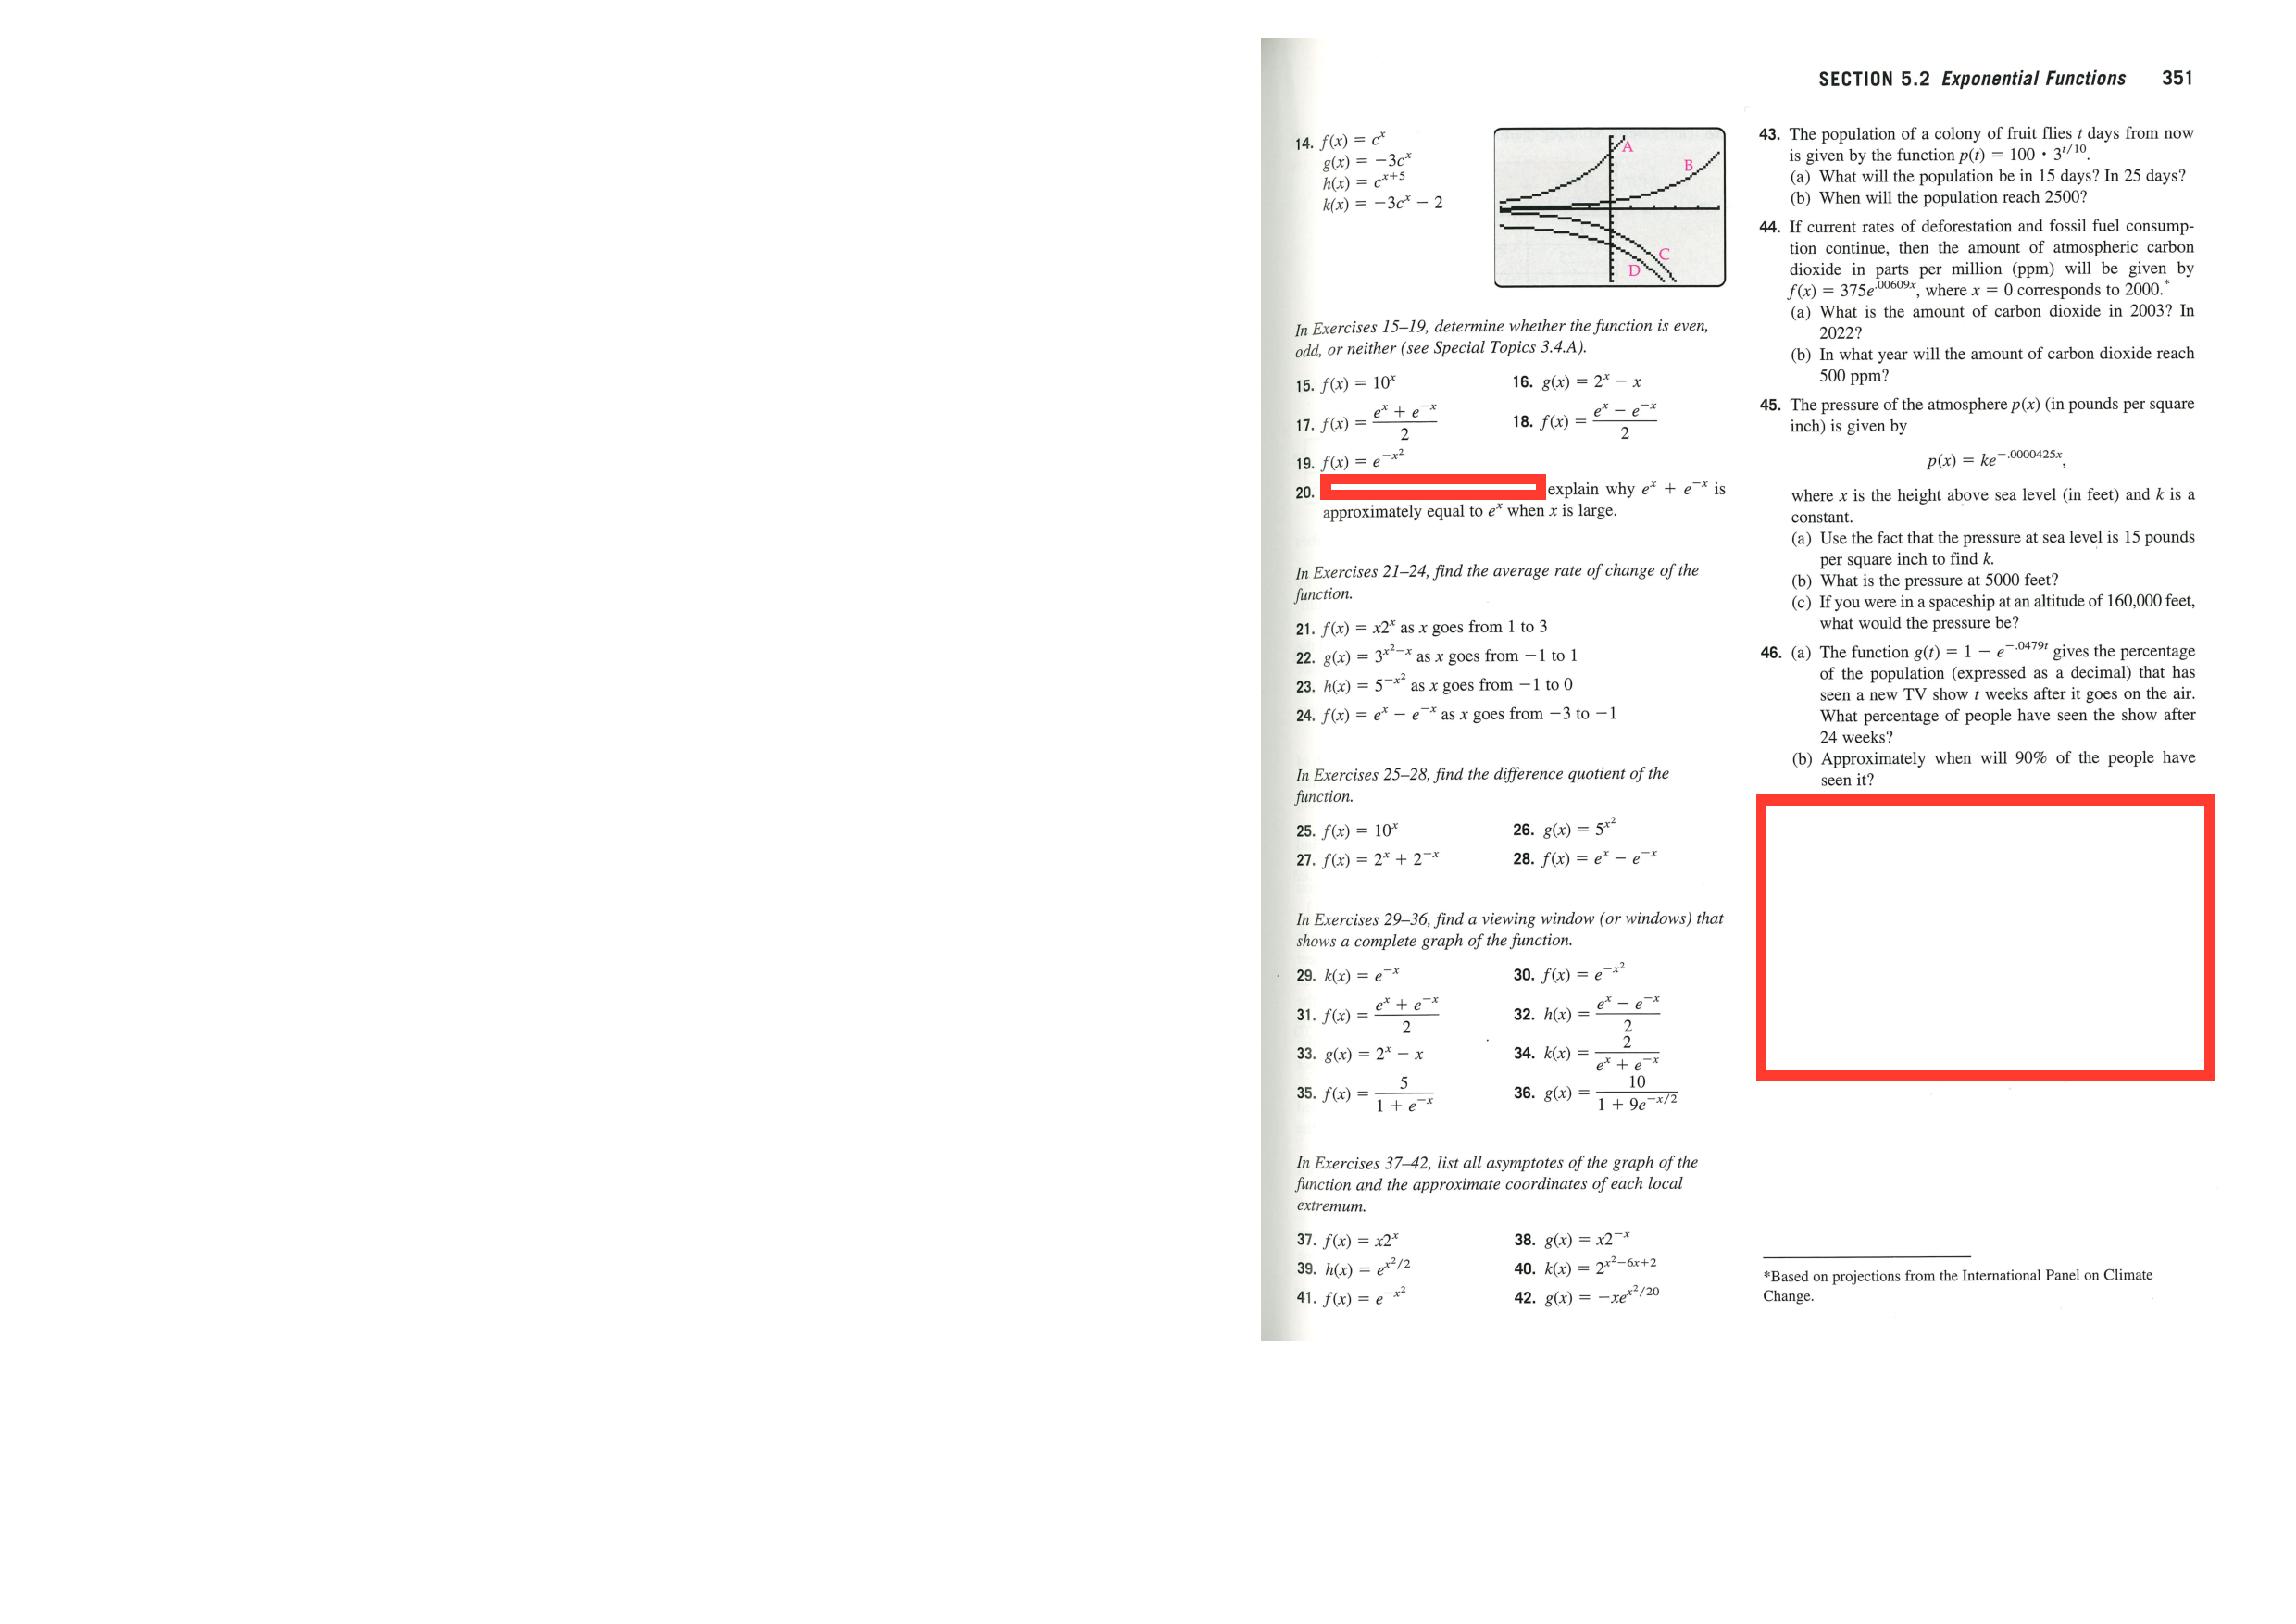
\includegraphics[width=\paperwidth]{\chapdir/0702xA.pdf}}
\newpage
\noindent\makebox[\textwidth]{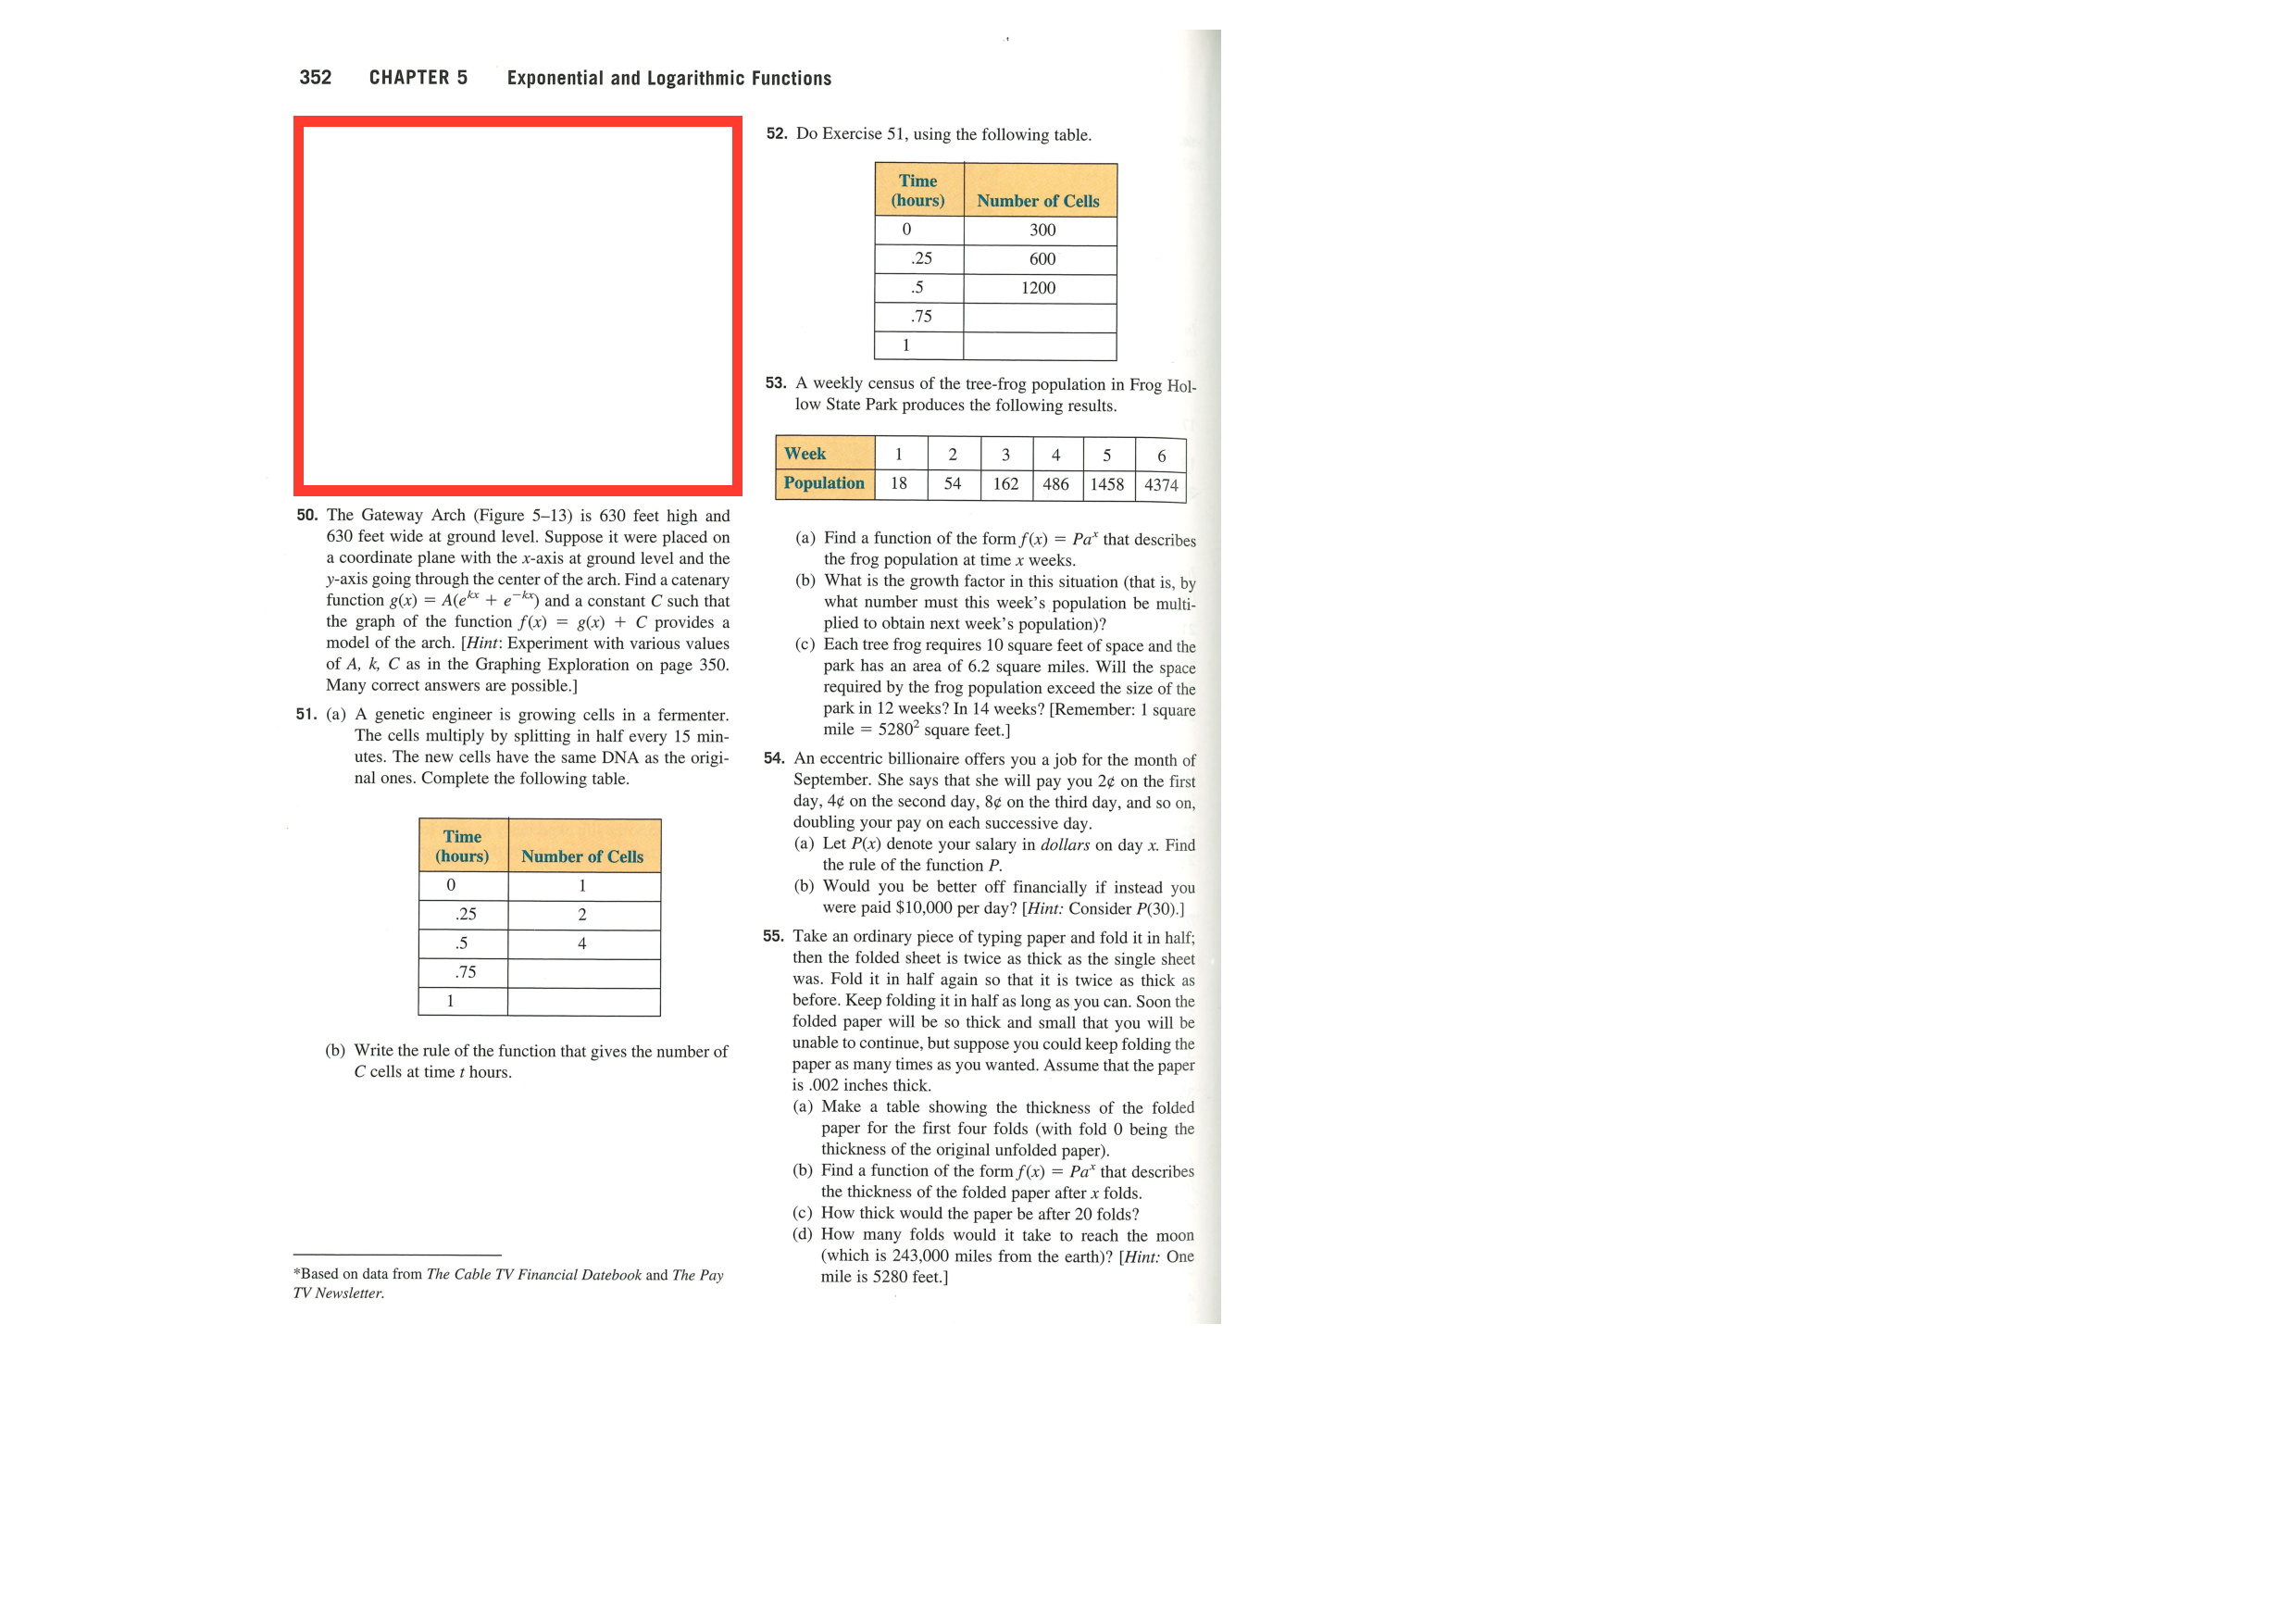
\includegraphics[width=\paperwidth]{\chapdir/0702xB.pdf}}
\newpage
\noindent\makebox[\textwidth]{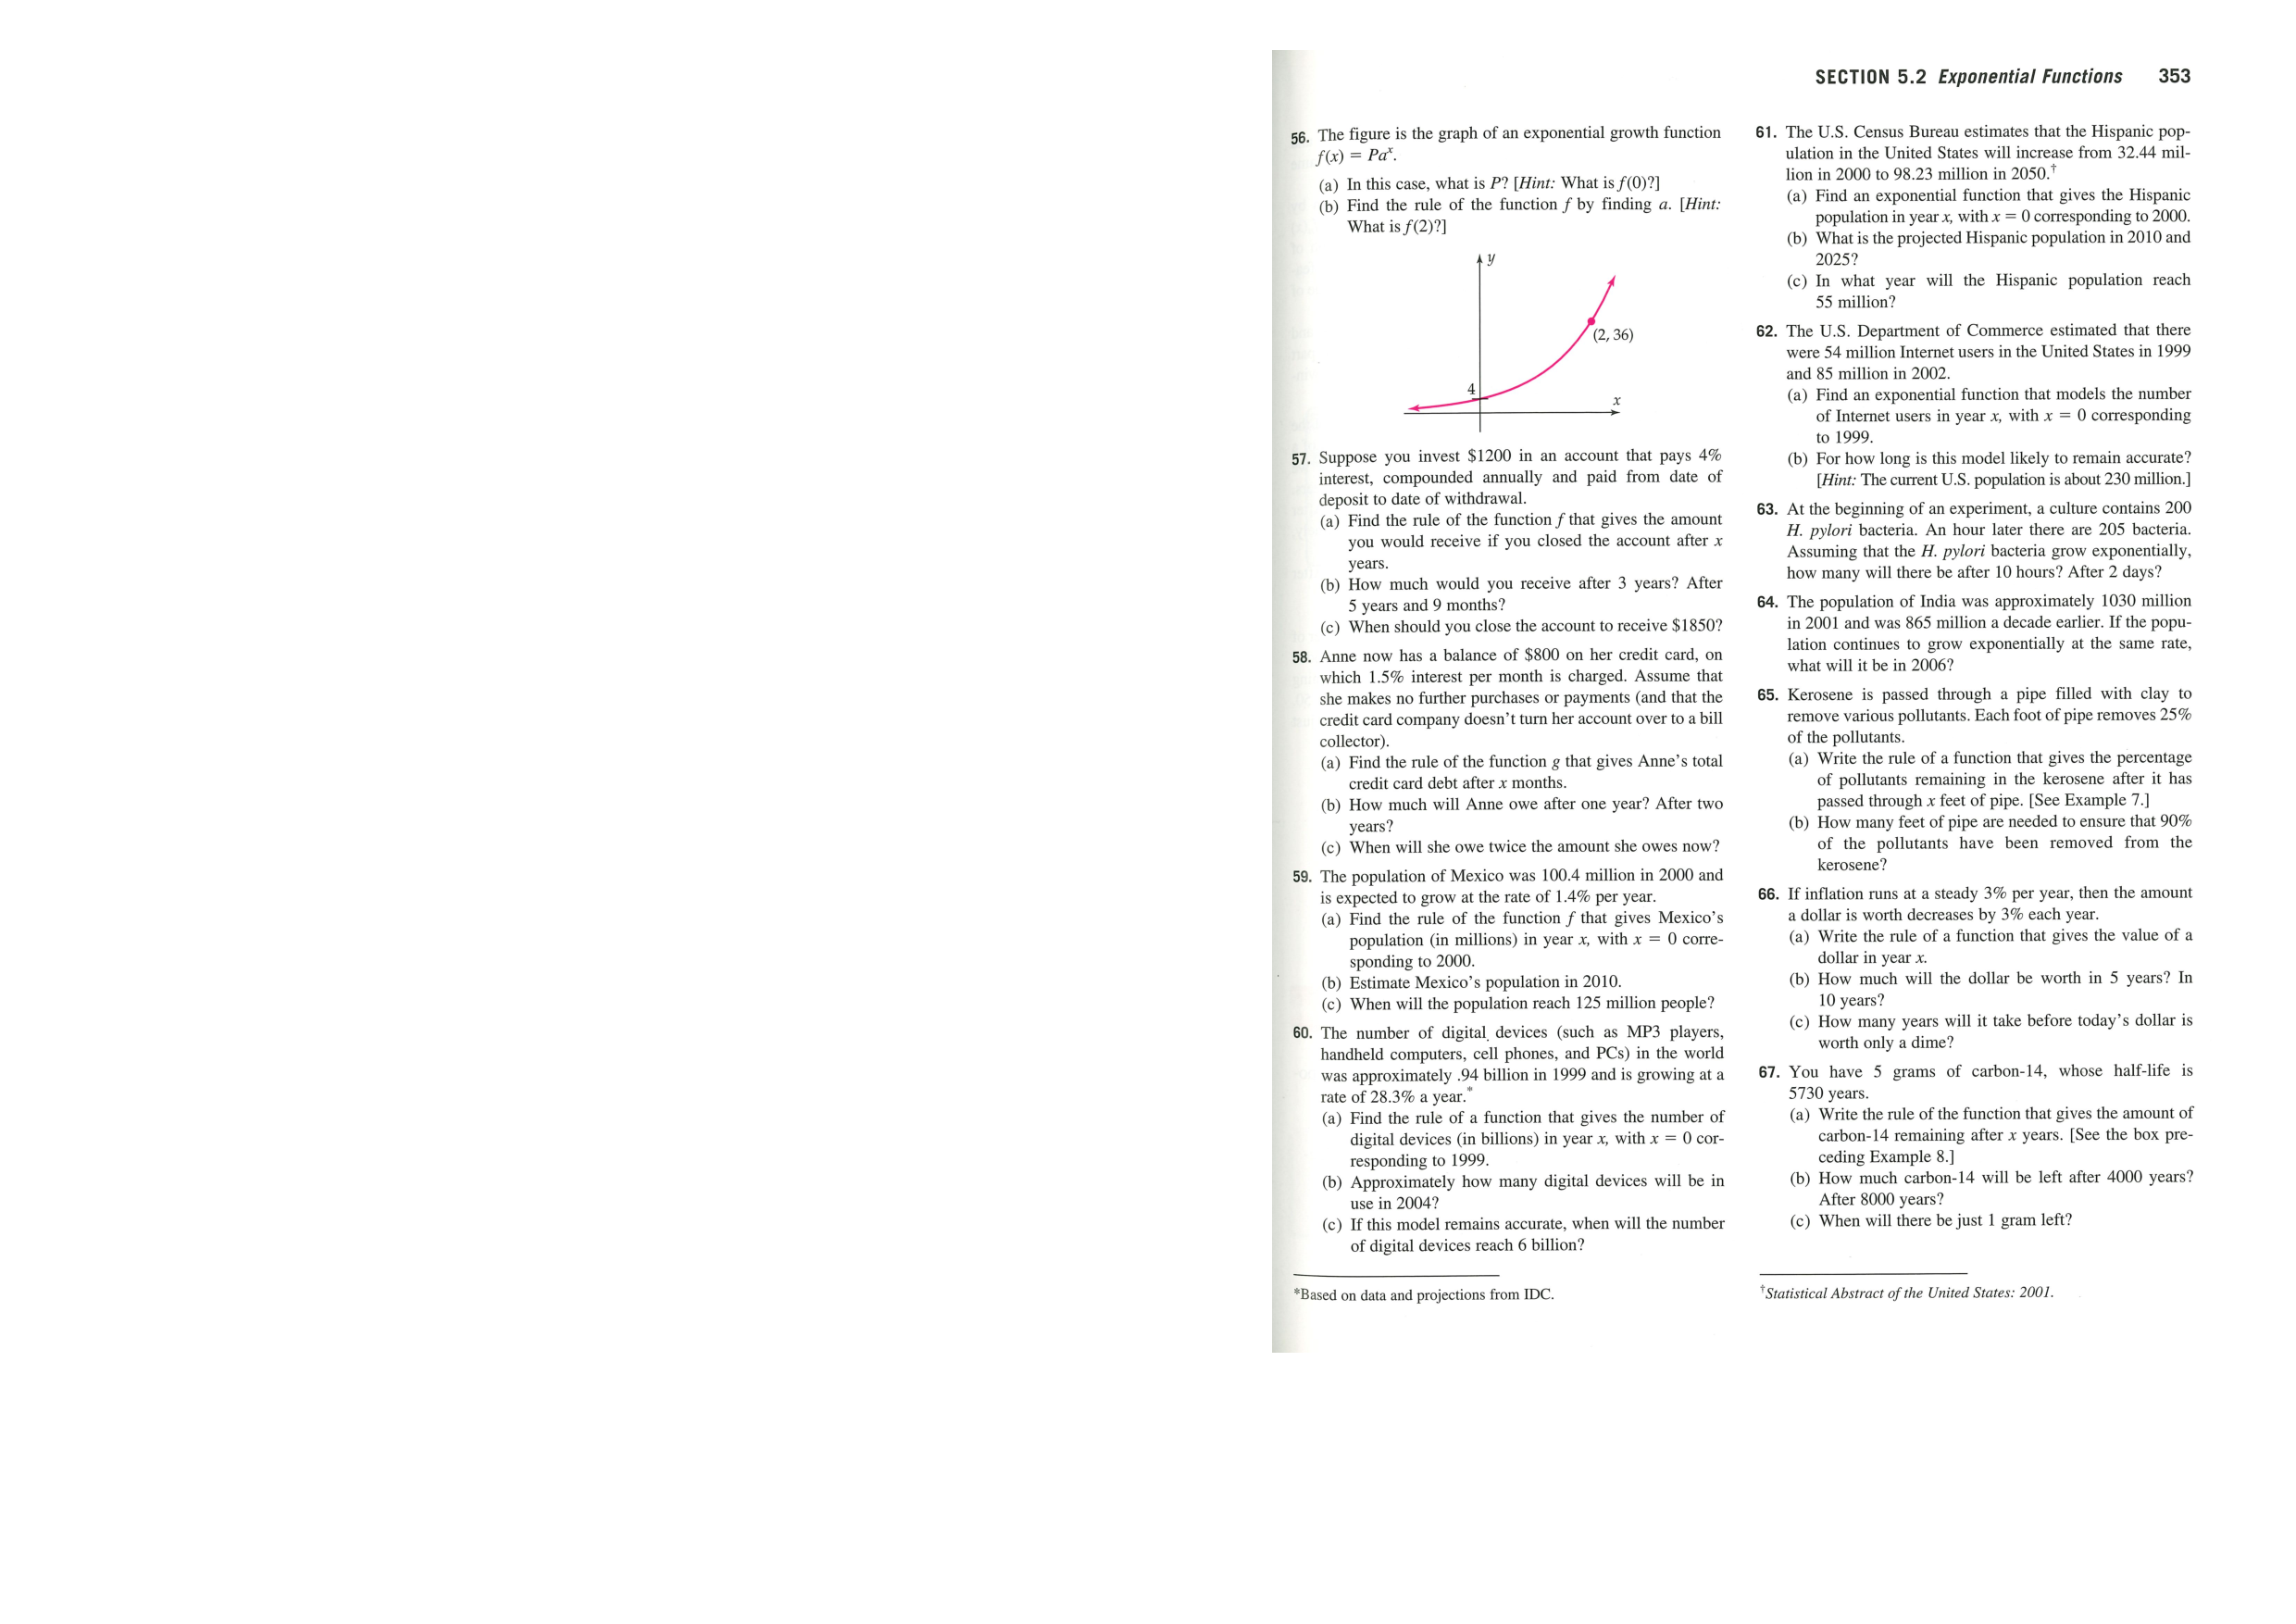
\includegraphics[width=\paperwidth]{\chapdir/0702xC.pdf}}
\newpage
\noindent\makebox[\textwidth]{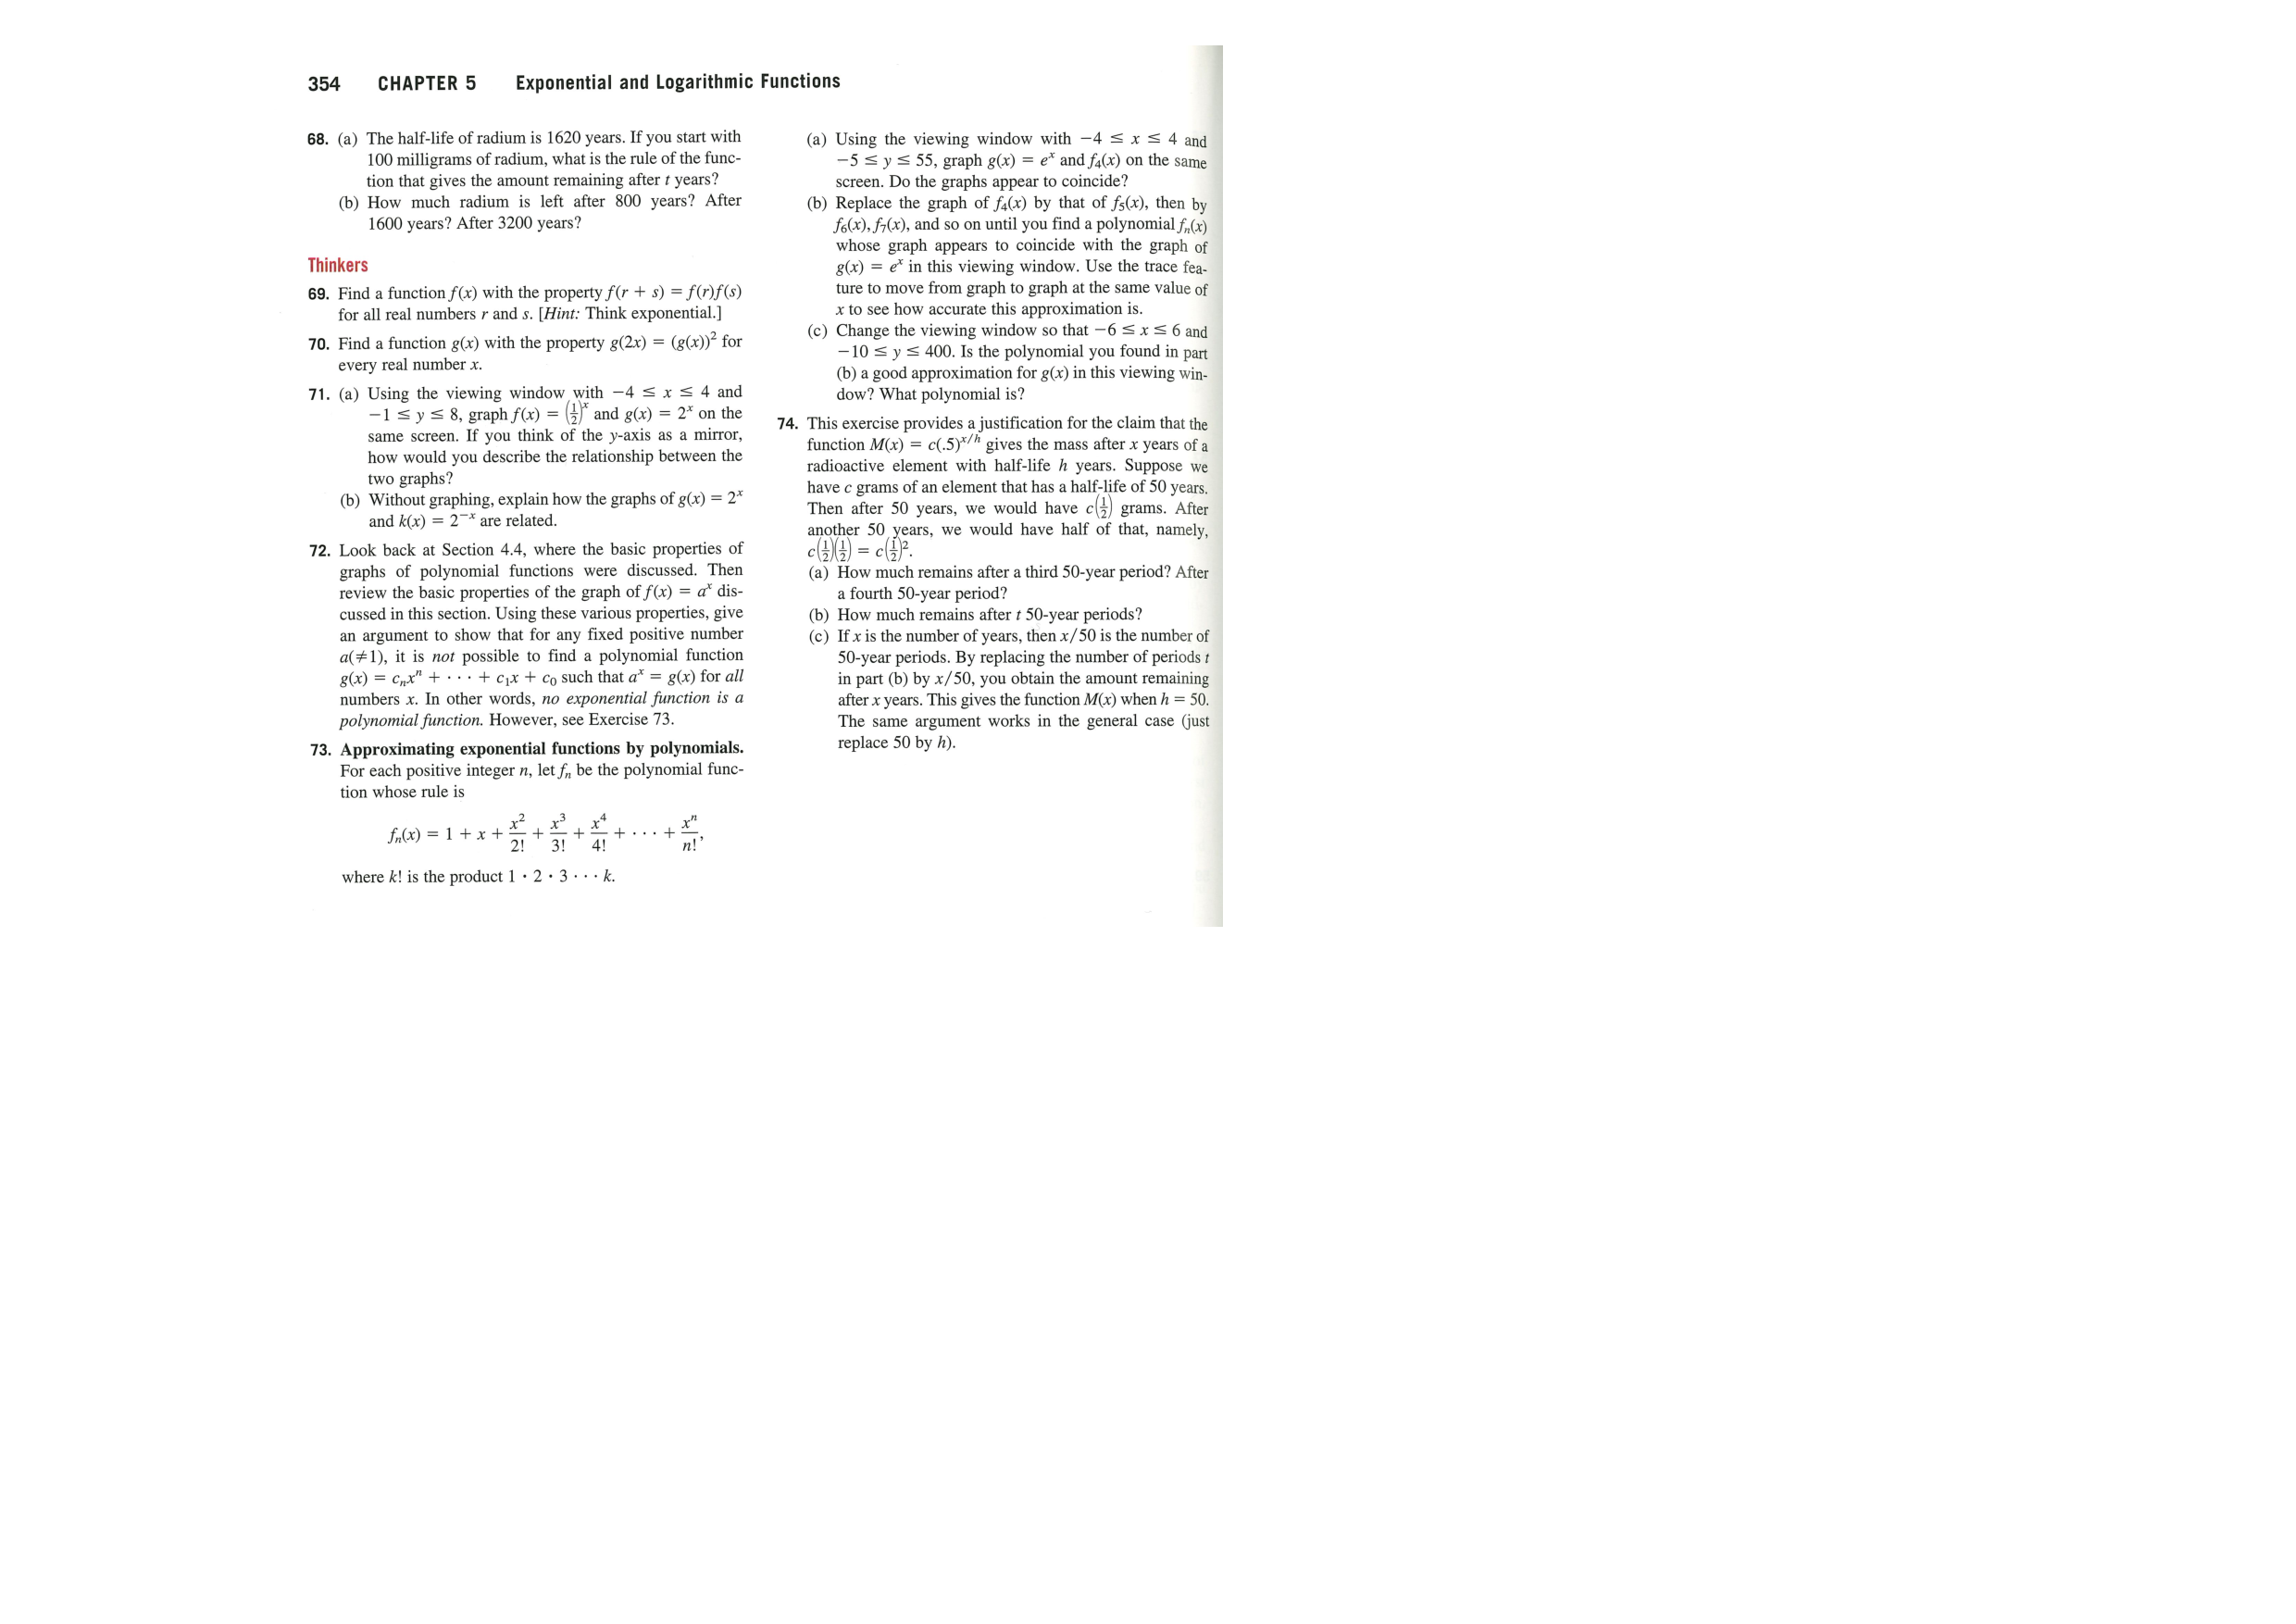
\includegraphics[width=\paperwidth]{\chapdir/0702xD.pdf}}



%									7 - 3
\newpage
\invisiblesection{Properties of Logs}
\marginlessinput{\chapdir/0703p}
\newpage
%!TEX root =  ../main.tex

\subsection{Like Powers}

\objective{Simply log expressions}


Whether we use the Triangle of Power or not, it is very powerful to recognize
that logs are simply the inverse of exponents.  Without this insight, expressions
like $\log_{10}{100} + \log_{10}{1000}$ would be very intimidating.  But with this
insight, we can paraphrase as we go in our minds: ``There is some exponent
to put on 10 and get 100.  Add to that, some exponent we put on 10 to get 
1000.  Adding exponents comes from multiplying bases, so this is the same as
$\log_{10}10000$.  That is asking the question, what exponent do we put on 10
to get 10,000?  5!''

We think it is even easier in Triangles, but we might show you both styles for
the time being:

$$
\tripow{10}{}{100} + \tripow{10}{}{1000} = \tripow{10}{}{10000} = 5
$$

In other words, two logs added, is the same as one long of a multiplication.  This
works for the inverse operation of subtraction: two logs subtracted is the same
as one log of a division.  Lastly, it also works for an exponent: the log of a number
with an exponent is the same as the exponent multiplied against the log of number.

Here, Triangle notation really shines superior, because notation like $\log_2{64^2}$
is confusing.  Does it mean $\log_2{64} \cdot \log_2{64}$ or $\log_2{4096}$, which
is the difference between 36 and 12?  How much clearer is

$$
\tripow{2}{}{\tripow{64}{2}{}} vs \tripow{\tripow{2}{}{64}}{2}{}
$$

Even more consequential is the two-fold possibilities for $2^{3^4}$.  Is that $(2^3)^4$
or $2^{(3^4)}$?  That is the difference between 4096 and $2^81$, the latter of which
is a 25 digit number!  But no one can make the same mistake with

$$
\tripow{\tripow{2}{3}{}}{4}{} vs \tripow{2}{\tripow{3}{4}{}}{}
$$


\subsection{Names}
There are some logs which occur so commonly, that they base is not written.  Normally,
the word ``log'' with no base written means $\log_{10}$.  Log base $e$ is very common,
and has its own symbol $\ln$.  This acronym comes from the French, \textit{log
natural}, since $e$ is the natural number.\footnote{In French, as in Spanish, adjective
most often follow their noun, not precede it.}  

Computer scientists most often used $\log_2$, which is called the binary log,
written lb.  In fact
in many disciplines, their flavor of log is the only one used, so it is assumed and the name
``log'' is written, which can fool outsiders into assuming $\log_{10}$.  For example,
Wolfram Alpha is fantastically powerful website for mathematics and other fields,
and so they use ``log'' to mean ``ln''!  We will not be so tricky, and you may assume
the solution to $\log{x}=2$ is 100.

\subsection{Change of Base}
Logs are amazing.  But given the rarity of most bases, it become necessary to ask,
Is there a way to convert them?  If we know how to re-write a log as an exponent,
and take an exponent as a multiplier, then we can:

\begin{align*}
	\log_b{a} & = c \\
	b^c &= a\\
	\ln{b^c} &= \ln{a}\\
	c \cdot \ln{b} &= \ln{a} \\
	c = \frac{\ln{a}}{\ln{b}} 
\end{align*}

Notice that it does not matter what base we chose in the third line.  $\ln$ ($\log_e$)
works just as well as $\log_{\pi}$.  This rearrangement to have an arbitrary
base is called the the Change of Base Formula.


\begin{derivation}{Change of Base Formula}
$$
\tripow{b}{}{a} = \frac{\tripow{c}{}{a}}{\tripow{c}{}{b}} \quad \text{a.k.a.} \quad
\log_b{a} = \frac{\log_c{a}}{\log_c{b}}
$$
\end{derivation}

\begin{derivation}{Negative Logarithm}
$$
\tripow{b}{}{1/y} = -\tripow{b}{}{y}  = \tripow{1/b}{}{y}
\quad \text{a.k.a.} \quad
\log_b{\frac{1}{y}} = -\log_b{y} = \log_{\frac{1}{b}}{y}
$$
\end{derivation}



Students often confusing ``the sum of logs'' with ``the log of a sum''.  What can we say
about $\log_b{(a+c)}$?  On the face of it, not much.  But through some creative manipulation,
one identity can be made, which is used in Probability Theory:


\begin{align*}
	\log_b{(a+c)} 	&= + \log_b{a} - \log_b{a} + \log_b{(a+c)}\\
				&= \log_b{a} + \log_b{(a+c)} - \log_b{a}\\
				&= \log_b{a} + \log_b{\frac{a+c}{a}} \\
				&= \log_b{a} + \log_b{1 + \frac{c}{a}}\\
	\tripow{b}{}{a+c} &= \tripow{b}{}{a} + \tripow{b}{}{\left(1 + \frac{c}{a}\right)}
\end{align*}

Lastly, we have already made with the Triangle of Power:

\begin{derivation}{P-Plus Logs}
$$
\tripow{m}{}{x} \pplus \tripow{n}{}{x} = \tripow{m\cdot{}n}{}{x}
\quad \text{a.k.a.} \quad
\log_m{x} \oplus \log_n{x} = \log_{mn}{x}
$$

$$
\tripow{m}{}{x} \pminus \tripow{n}{}{x} = \tripow{m\div{}n}{}{x}
\quad \text{a.k.a.} \quad
\log_m{x} \pminus \log_n{x} = \log_{\frac{m}{n}}{x}
$$

$$
\tripow{\tripow{m}{n}{}}{}{x} = \frac{\tripow{m}{}{x}}{n}
\quad \text{a.k.a.} \quad
\log_{m^n}{x} = \frac{1}{n}\log_m{x}
$$
\end{derivation}

\newpage
\begin{defproblem}{0703:All6}
\begin{onlyproblem}
There are six ways to arrange $x$ and $y$ and $9$
on the Triangle of Power (or on $a^b=c$, $\sqrt[a]{b}=c$, or $\log_a{b}=c$).
Write down all six and rearrange each into a form
enterable in your TI-8*.  
\begin{enumerate}
\item Graph each under ZOOM-STANDARD and in your notebook.
\item Find two lattice points on each.
\item How many lattice points are there on each?
\item Which are inverses of each other?
\item Which are reciprocals of each other?
\item Find reciprocals of the others
\end{enumerate}
\end{onlyproblem}
\begin{onlysolution}
\begin{enumerate}
\item graphs
\item yup
\item infinite, infinite, infinite, two, infinite, two
\item roots and powers, logs and exponents, the other two
\item $9^y=x$ and $x^y=9$
\end{enumerate}
\end{onlysolution}
\end{defproblem}



\begin{defproblem}{0703:Logproofs}
\begin{onlyproblem}
True or False?
\begin{enumerate}
\item $-\log_b{x} = \log_x{b}$ 
\item $\ln{|x|} = |\ln{x}|$
\item $\log_{\sqrt{3}}{27} =6$
\item $e^{x\ln{x}} = x^x$ when $x>0$
\item $\sqrt{\log{x}} = \log{\sqrt{x}}$
\item $x\log_x{x^x} = x^2$
\item $\log_{\sqrt{5}}{\frac{1}{125}} = -4$
\item ${2^{\frac{1}{2}^{\frac{1}{2}^{\iddots}}}} = 1$
\end{enumerate}
\end{onlyproblem}

\begin{onlysolution}
\begin{enumerate}
\item true
\item false
\item true
\item false
\item false
\item true
\item false
\item true, but the vagaries of regular notation could make it $2^0=1$
\end{enumerate}
\end{onlysolution}
\end{defproblem}



\begin{defproblem}{0703:SolveLogs}
\begin{onlyproblem}
Solve for $x$.  Rewriting with the Triangle of Power is very helpful
\begin{enumerate}
\item $\log_x{(x+6)}=2$
\item $\log{\left(\log{\left(\log{(x+1)} \right)} \right)} = 0$ 
\end{enumerate}
\end{onlyproblem}
\begin{onlysolution}
\begin{enumerate}
\item 3 or -2
\item 999,999,999
\end{enumerate}
\end{onlysolution}
\end{defproblem}


\begin{defproblem}{0703:SimplifyLogs}
\begin{onlyproblem}
Prove
\begin{enumerate}
\item $\ln{\left(\frac{\sqrt{x}}{x}\right)} + \ln{\sqrt[4]{ex^2}}=0.25$
\item $\log_b{a} = \frac{1}{\log_a{b}}$
\item $\log_b{x} \cdot{} \log_x{y} = \log_b{y}$
\item $x^{\log_b{y}} = y^{\log_b{x}}$  (Hint, rewrite $x$ as $b$ to a certain power)
\item $\log_b{y^x} = \log_{\sqrt[x]{b}}{y}$
\item $\log_y{x^b} = -\log_x{y^b}$
\item $2^{-\log_x{2}} = \sqrt[-\log_2{x}]{2}$
\end{enumerate}
\end{onlyproblem}
\begin{onlysolution}
\begin{enumerate}
\item 1/4
\end{enumerate}
\end{onlysolution}
\end{defproblem}


\begin{defproblem}{0703:DesribeTri}
\begin{onlyproblem}
Describe the difference between $\log_5{x} + 2$ and $\log_5{(x+2)}$
and show how Triangle notation might help
\end{onlyproblem}
\begin{onlysolution}
Up 2 vs left 2
\end{onlysolution}
\end{defproblem}

\begin{defproblem}{0703:DescribeCalclog}
\begin{onlyproblem}
Using your TI-8* and reasoning skills, find the asymptotes,
hole(s), and local extrema of 
\begin{enumerate}
\item $y=x\log{x^2}$
\item $y=x^2\ln{|x}$
\item $y=\sqrt[\log_{x^2}{9}]{|x|}$
\item $y=\log_{|x|}{9}$
\end {enumerate}
\end{onlyproblem}
\begin{onlysolution}
\begin{enumerate}
\item hole at zero
\end{enumerate}
\end{onlysolution}
\end{defproblem}





\endinput

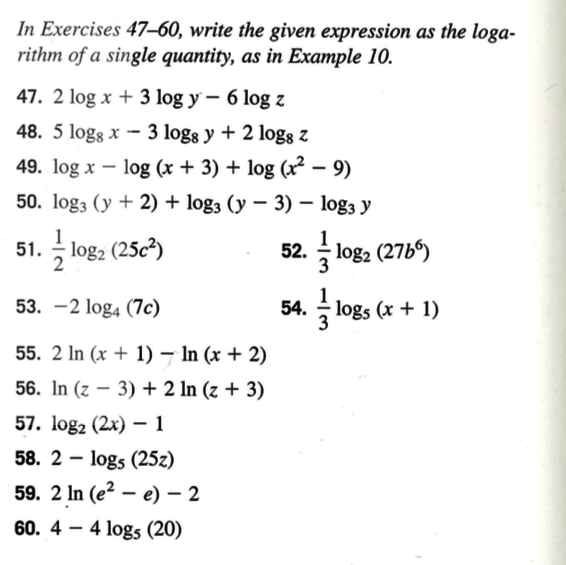
\includegraphics[scale=0.5]{ch07/0703xA.png}
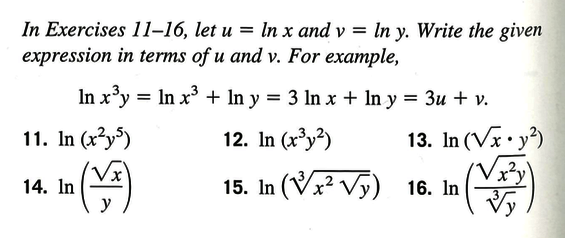
\includegraphics[scale=0.5]{ch07/0703xB.png}

%									7 - 4
\newpage
\invisiblesection{Log Equations}
\marginlessinput{\chapdir/0704p}
\newpage
%!TEX root =  ../main.tex

\subsection{Exponential Equations}

\objective{Solve exponential/logarithmic equations through a variety of techniques}


Whatever function we are dealing with, if $f(x)=f(3)$ then $x$ must equal 3.  This is true
if $f(x)$ is a logarithmic, exponential or other kind of function.  So, if $\log_{\pi}(x+3) =
\log_{\pi}{7-x}$, then $x+3 = 7 - x$ and $2x = 4$, so $x$ must equal 2.  Similarly,
if $3^{2x+1} = 3^7$ then $2x+1 =7$ and $x=3$.  These are the most basic kinds of
exponential equations.

You are probably pretty good at spotting when numbers are related via multiplication
and division because of so many years of practicing such arithmetic.  $56x+49=0$ should
leap out to you as $7(8x+7)=0$ or even $x=-\frac{7}{8}$ because you have known
your seven times table for so many years now.  Exponents are not memorized to the
same extent --- and nor should they be --- but perhaps you might consider expanding your
familiarity with them just a little more.  The return on investment is pretty low after cubes,
but you will be pleasantly surprised at the added reach knowing the numbers on the following
table will give you:

$$
\begin{matrix} 
2 & 4 & 8 & 16 & 32 \\ 
3 & 9 & 27 & 81 & 243 \\ 
4 & 16 & 64 & 256 & 1024 \\ 
5 & 25 & 125 & 625 &  \\ 
6 & 36 & 216 &  &  \\ 
7 & 49 & 343 &  &  \\ 
8 & 64 & 512 &  &  \\ 
9 & 81 & 729 &  &  
\end{matrix}
$$

\begin{example}{Exponential Base Manipulation}
\exProblem
Solve $9^{x+1}=\left(\frac{1}{27}\right)^{2x}$.

\exSolution
With a familiarity with exponents, we see that both numbers are power of 3.  We can 
re-write each base to show this, and use the same equality principle as before.
\begin{align*}
	9^{x+1} &= \left(\frac{1}{27}\right)^{2x}\\
	(3^2)^{x+1} &= (3^{-3})^{2x}\\
	3^{2x+2} &= 3^{-6x}\\
	2x + 2 &= -6x\\
	8x &= -2\\
	x &= -\frac{1}{4}
\end{align*}
\end{example}

\begin{example}{Logarithmic Base Manipulation}
\exProblem
Solve $\log_7{x} = \log_{49}{2x}$.

\exSolution
There are lot of transformation we could try at this point which would be valid.
Let us consider how we can make both sides have a logarithmic base of 49.
$\log_7{7} = \log_{49}{49}$, which shows that is you square the base, you must square
what you are taking the log of.  This will allow us to rewrite the equation and solve.
\begin{align*}
	\log_7{x} &= \log_{49}{2x}\\
	\log_{49}{x^2} &= \log_{49}{2x}\\
	x^2 &= 2x \\
	x^2 - 2x &= 0\\
	x(x-2) &= 0\\
	x &= \{0, 2\}
\end{align*}
If we check our two solutions, however, we find a contradiction.  $\log_b{0}$ does
not exist: there is no exponent you can raise a number to and get 0.  We can check that
2 works as a solution in our TI-8*.  (Newer TI-8*'s have a LOGBASE function under MATH, 
but everyone can check by typing $\frac{\log{2}}{\log{7}}$ etc.)
\end{example}

\begin{example}{Combining Logs}
\exProblem
Solve for $x$: $\log_4{(x+10)}+\log_4{(x+34)}=4$

\exSolution
We can (must) combine the two logs, in order to make the problem simpler.
\begin{align*}
	\log_4{(x+10)(x+34)} &= 4\\
	\log_4{x^2+44x+340)} &= 4\\
	4^4 &= x^2+44x+340\\
	0 &= x^2+44x+340-256\\
	0 &= (x+2)(x+42)
\end{align*}
Of the two solutions, only -2 works in the original problem; -42 does not
\end{example}

\subsection{Substitution}
Finally, there are some problems which do not yield to combination, manipulation, or
changing log-form.  These problems require substitution.  For example, nothing in 
$e^{2x}+5e^x=1$ seems to fit what we have so far described.  We cannot combine
any terms of the left, so we must ``explain away'' for a moment the troublesome
exponents.  We pick a variable to represent what we cannot deal with: $e^x$.  

The problem now becomes $u^2+5u=1$.  This is not magic: we must un-substitute at the
end, or else we are solving a different problem.  But the magical aspect is that we can now
see that this is a quadratic problem.  $u^2+5u-1=0$ does not yield to factoring, so
we must resort to the Quadratic Formula.

$$
u=\frac{-5\pm\sqrt{29}}{2}
$$

We check with the TI-8*, and the ```plus'' solution is positive, while the ``minus'' one is not.
Since $u$ is really just a cipher for $e^x$, we need only the positive solution.  This means
$e^x=\frac{-5+\sqrt{29}}{2}$ or $x=\ln{-5+\sqrt{29}}-\ln{2}$, which is around -1.65.

\newpage
\subsection{Exercises}
In kuta


%									7 - 5
\newpage
\invisiblesection{Logistic Curves}
\subsection{Problems}
\noindent\makebox[\textwidth]{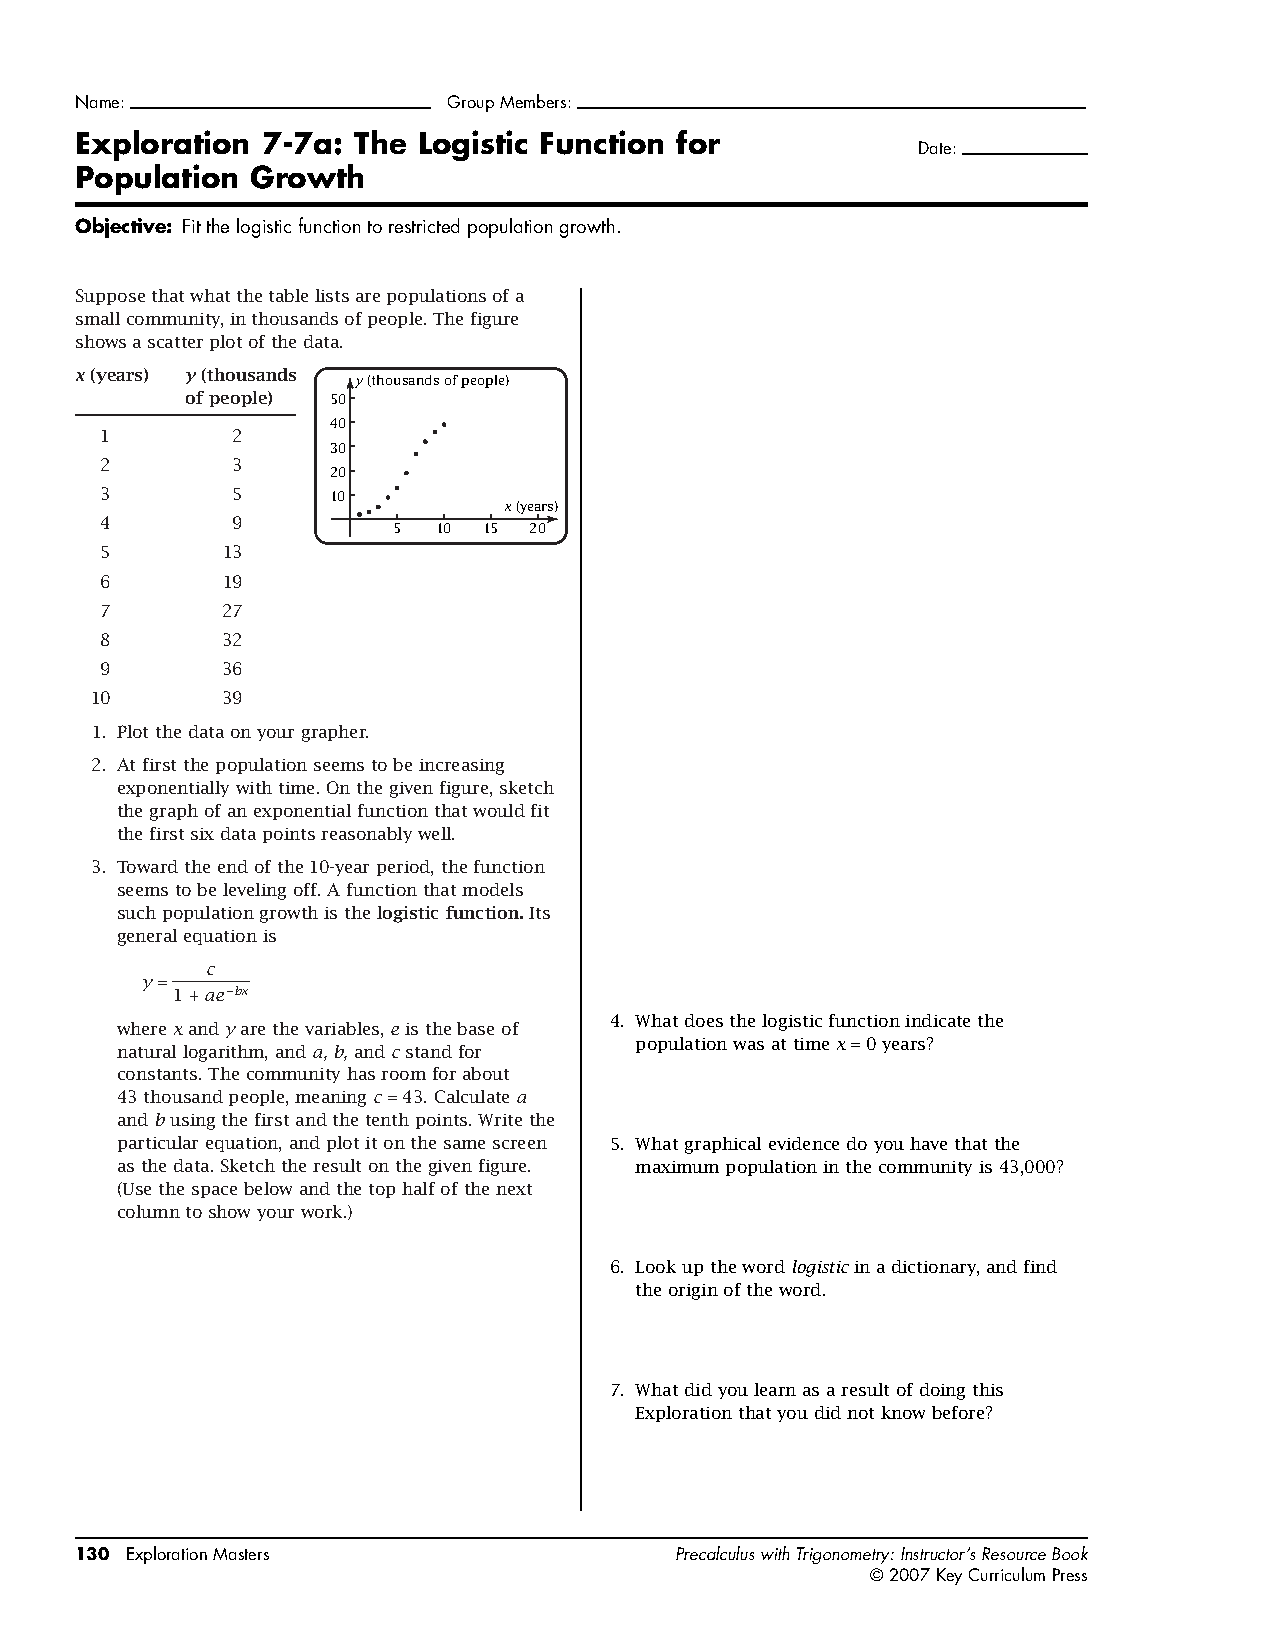
\includegraphics[width=\paperwidth]{ch07/0705p.pdf}}
\newpage
%!TEX root =  ../main.tex

\subsection{Restrained Growth}

\objective{Create and use logistic curves}


Exponential growth can rarely be carried on for long.  Bacteria fill the petri dish, 
bunnies eat all the grass, and the shower-water has a maximum heat it can 
reach.  In every case, the is a constraint, a ceiling value that the population 
cannot grow beyond.  Typically, it is approached asymptotically.  This means there are
two horizontal asymptotes.  The left half of the graph is concave up (exponential
growth) and the right half is concave down (logarithmic growth).  

How can these graphical quantities be achieved algebraically?  What can 
be done to $y=e^x$ to make it have a horizontal asymptote?  As we saw last
chapter, rational functions have horizontal asymptotes at the level of the ratio
of the numerator to the denominator ``at infinity''.  So we need to create a 
denominator.  But we don't want the denominator to ever equal 0, lest we
create a vertical asymptote.  Dividing by $e^x$ is almost right.  Let's make it
$e^x+1$.

$$
f(x) = \frac{e^x}{e^x+1}
$$

\begin{figure}[h]
\begin{centering}
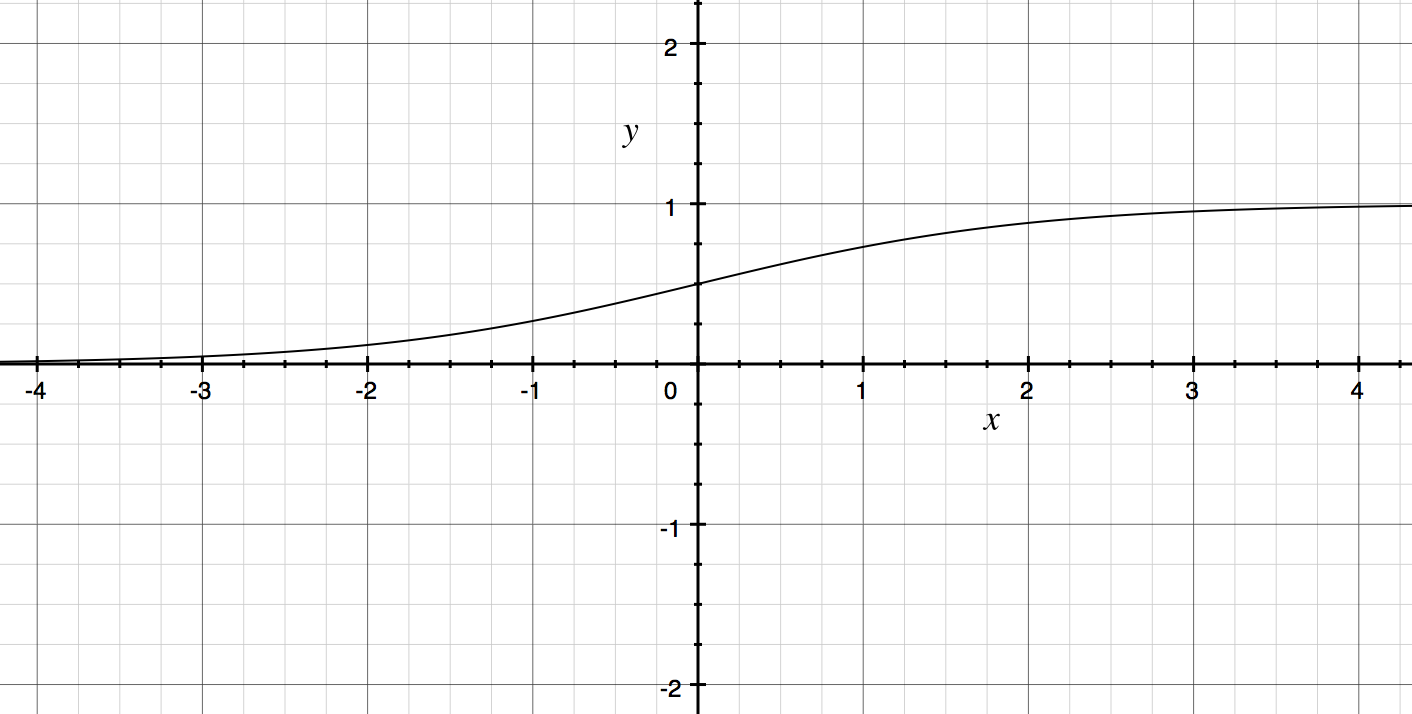
\includegraphics[scale=0.5]{basicalogistic}
\caption{A basic logistic curve}
\end{centering}
\end{figure}

That worked out nicely, but it made our equation slightly more complicated
than we might otherwise like.  If we want to do any inside transformation (e.g.
shift left/right, widen/narrow) then we will need to modify $x$ in two places.  Can
we consolidate the $x$ to be in only one place?  What could we do to the
numerator and denominator ?

Dividing top and bottom by $e^x$ will cancel the two terms with $x$ in them.
Furthermore, we can eliminate the need for complex fraction by changing
a denominator under 1 to be a negative exponent.

$$
f(x) = \frac{1}{1+e^{-x}}
$$

Notice which numbers control the behavior of the graph.  The 1 in the numerator
is the maximum height of the graph, which typically called $c$ for ceiling. If we
insert a multiplying constant next to $x$ in the exponent, it will contract the
graph in the $x$-direction, making the curve of the S steeper.  If we insert
a multiplying constant next to x, it will shift the turning point to the right.  No
matter what we do, the inflection point will occur half-way up.

$$
f(x) = \frac{c}{1+ae^{-bx}}
$$

\subsection{Regression}
The TI-8* has a LOGISTICREG function which is excellent for computing
regressions of this kind, and outputs functions of the kind already discussed.
However, if we need to make an equation ourselves by hand, $e$ is slightly
awkward number to use.  Algebra manipulation is much easier with this
equation:

$$
f(x) = \frac{c}{1+ab^{-x}}
$$

\newpage
\subsection{Exercises}
\noindent\makebox[\textwidth]{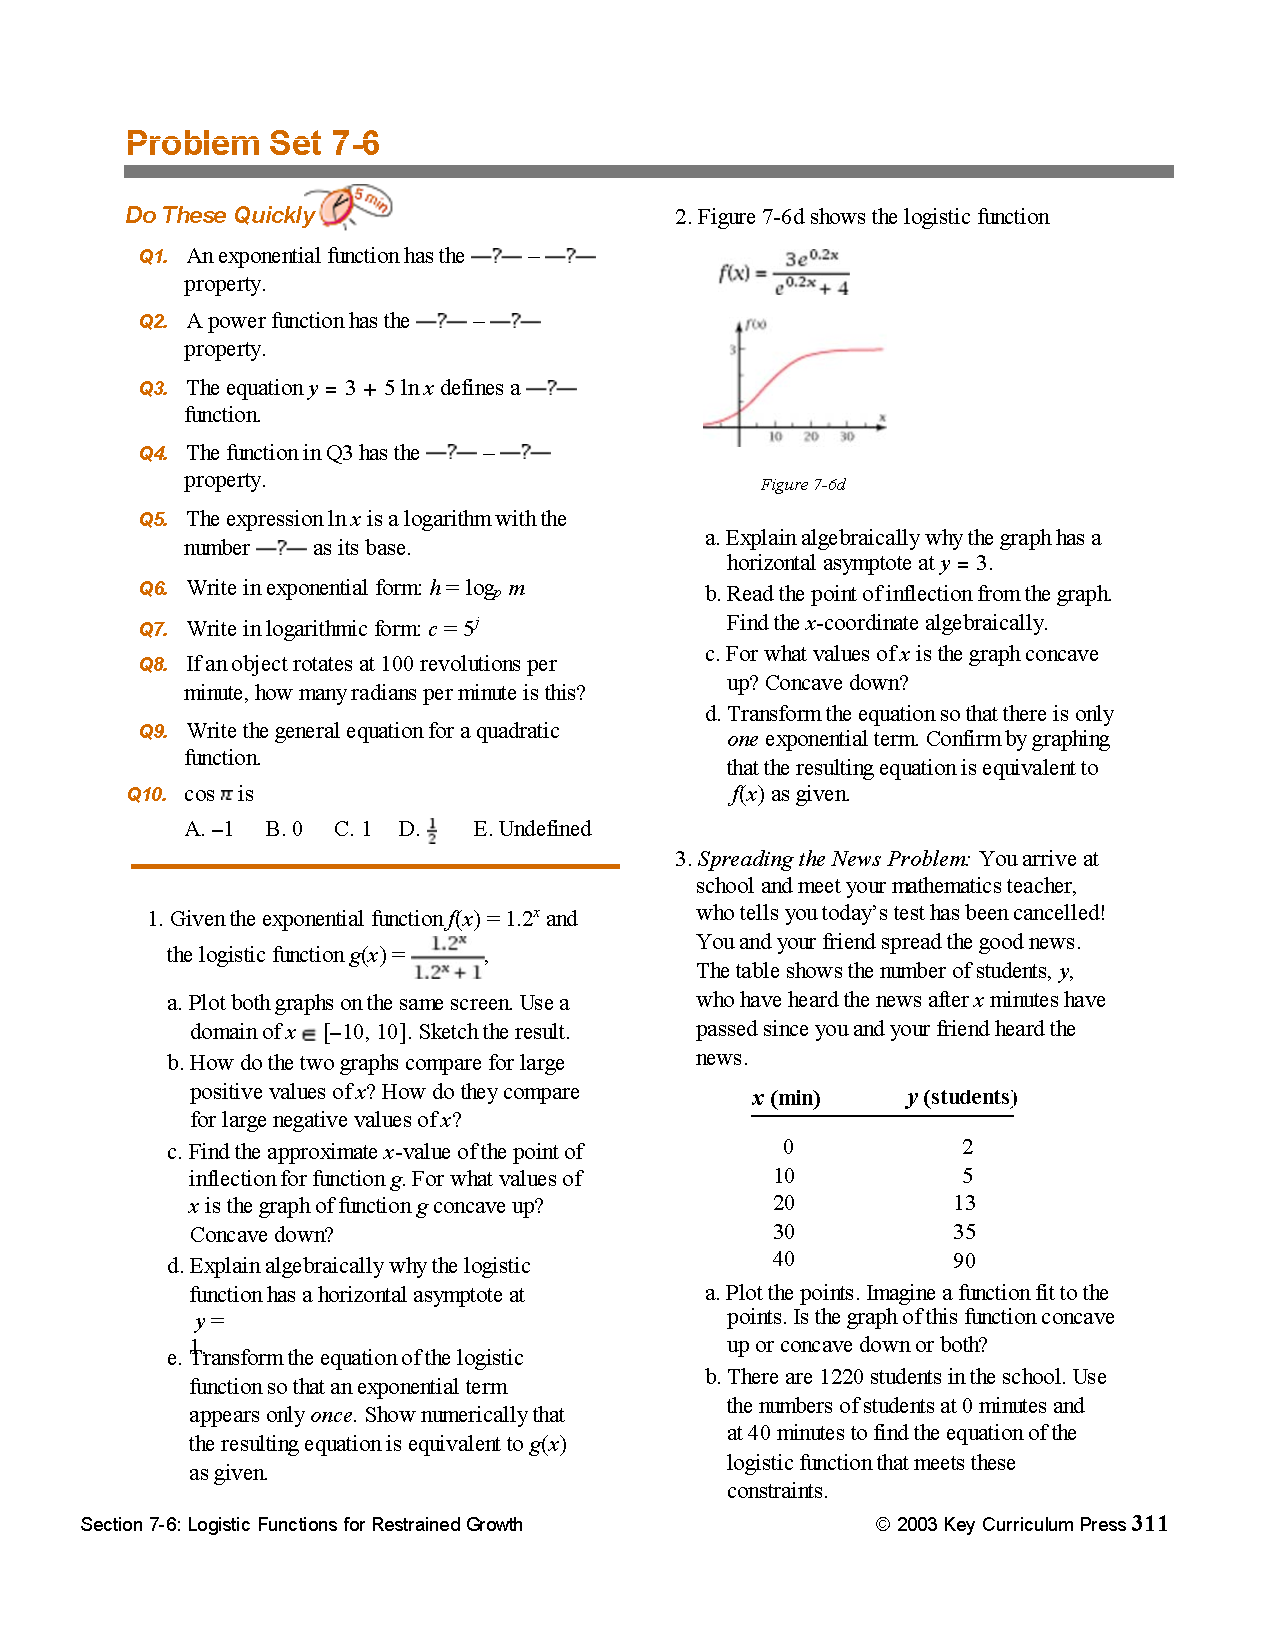
\includegraphics[width=\paperwidth]{ch07/0705xA.pdf}}
\newpage
\noindent\makebox[\textwidth]{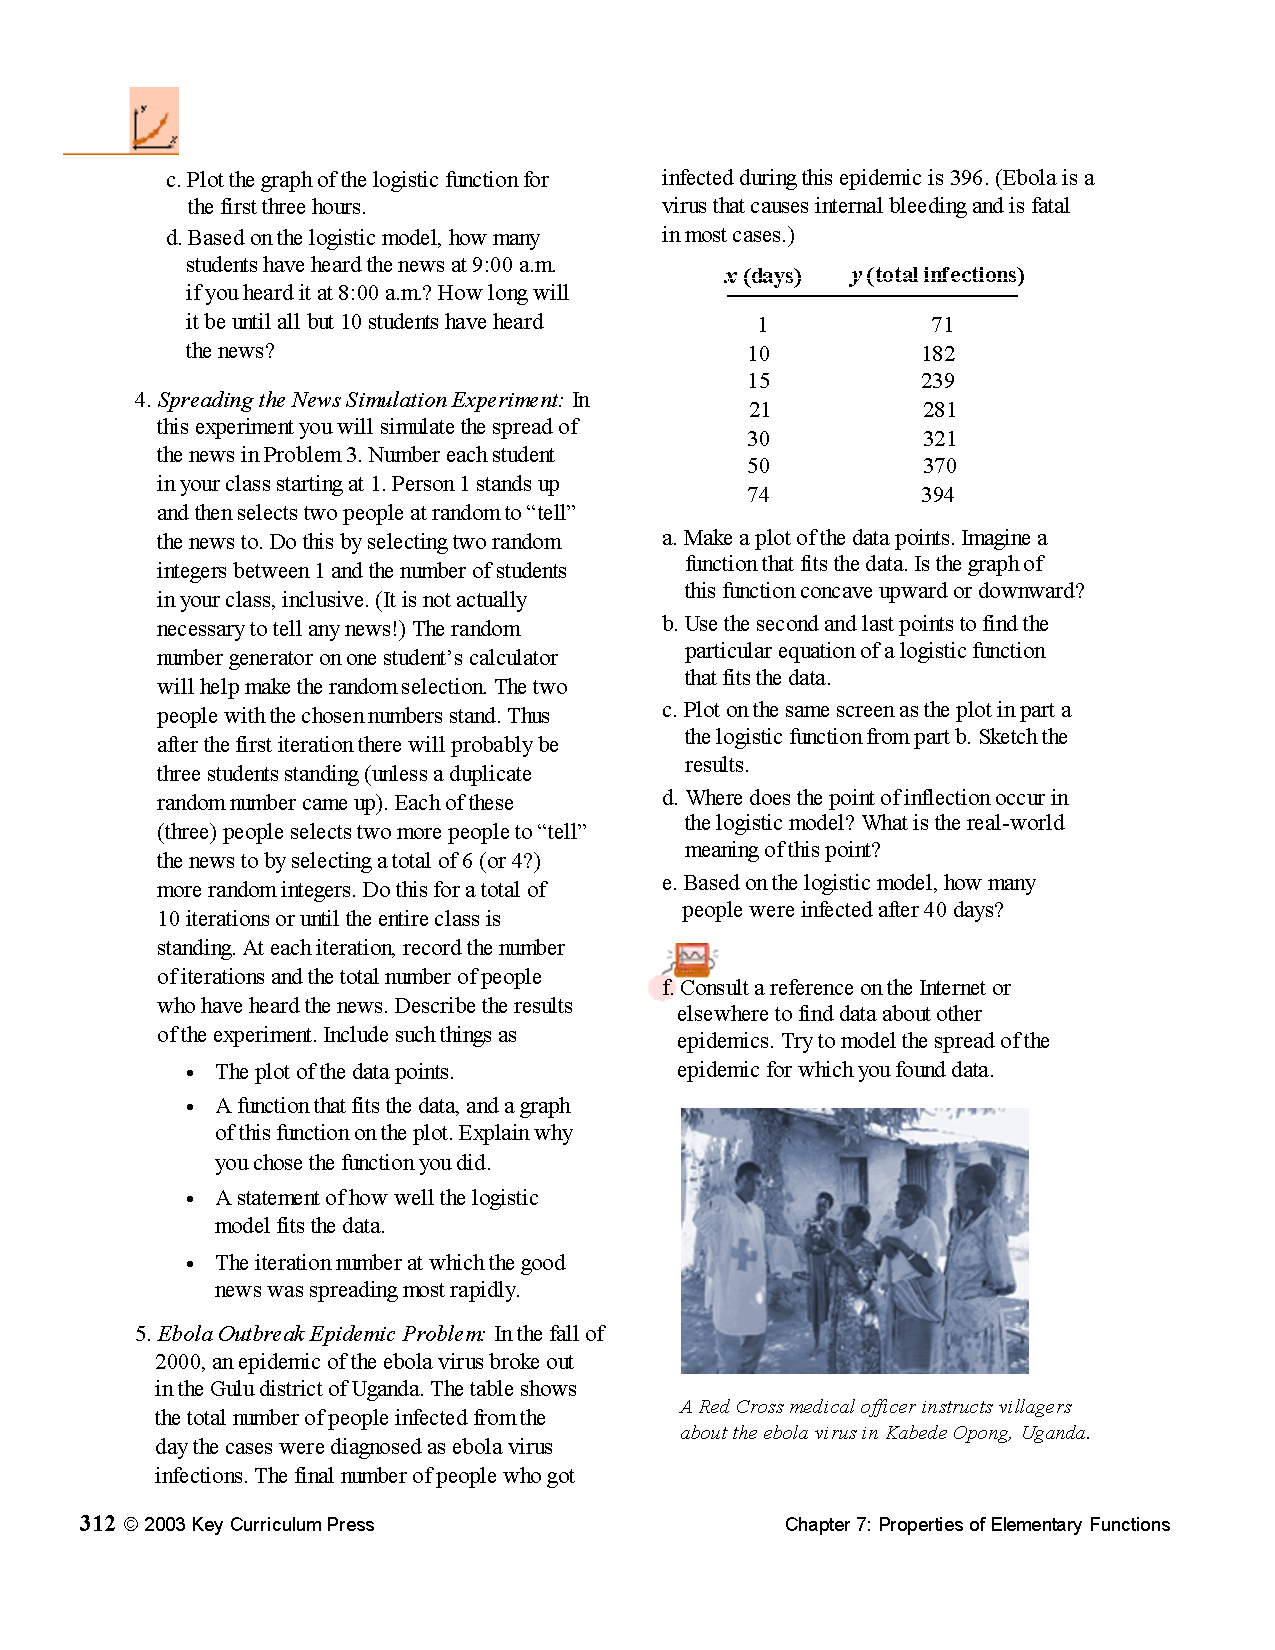
\includegraphics[width=\paperwidth]{ch07/0705xB.pdf}}
\newpage
\noindent\makebox[\textwidth]{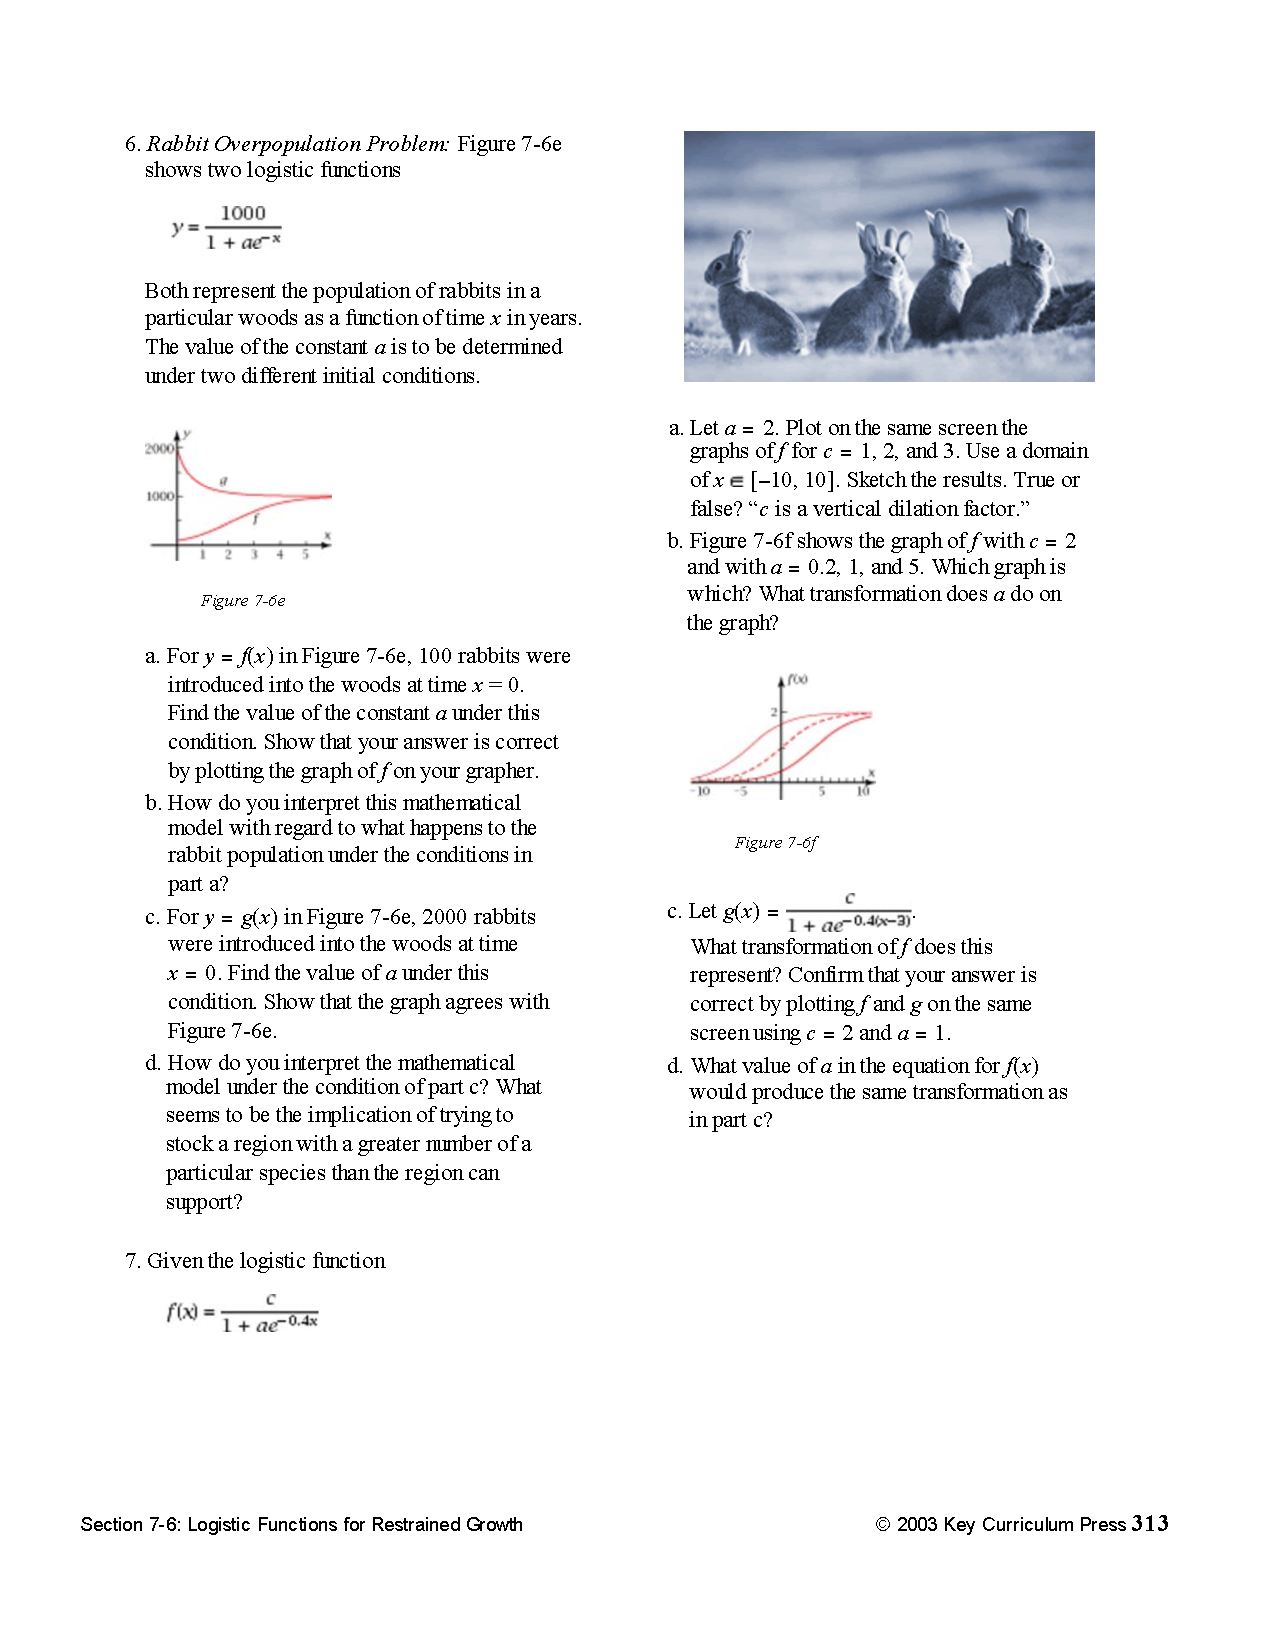
\includegraphics[width=\paperwidth]{ch07/0705xC.pdf}}


%									7 - 6
\newpage
\section{Review}
\subsection{Chapter Review}
%!TEX root =  ../main.tex

\subsection{Hold Power Steady}
\subsubsection{Vary Root}
\begin{align*}
\tripow{m}{}{x} \pplus \tripow{n}{}{x} &= \tripow{m\cdot{}n}{}{x} & \quad
	\log_m{x} \pplus \log_n{x} & = \log_{m\cdot{}n}{x} \\
\tripow{m}{}{x} \pminus \tripow{n}{}{x} &= \tripow{m \div n}{}{x} & \quad
	\log_m{x} \pminus \log_n{x} & = \log_{m \div n}{x} \\
\tripow{\tripow{m}{n}{}}{}{x} &= \frac{1}{n} \tripow{m}{}{x} & \quad
	\log_{m^n}{x} &= \frac{1}{n}\log_m{x}\\
\end{align*}


\subsubsection{Vary Exponent}
\begin{align*}
\tripow{}{m}{x} \cdot \tripow{}{n}{x} &= \tripow{}{m\pplus{}n}{x} & \quad
	\sqrt[m]{x} \cdot \sqrt[n]{x} &= \sqrt[m\pplus{}n]{x} \\
\tripow{}{m}{x} \div \tripow{}{n}{x} &= \tripow{}{m\pminus{}n}{x} & \quad
	\sqrt[m]{x} \div \sqrt[n]{x} &= \sqrt[m\pminus{}n]{x} \\
\tripow{}{m\cdot{}n}{x} &= \tripow{}{n}{\tripow{}{m}{x}} & \quad
	\sqrt[m\cdot{}n]{x} &= \sqrt[n]{\sqrt[m]{x}} \\
\end{align*}

\subsection{Hold Exponent Steady}
\subsubsection{Vary Power}
\begin{align*}
\tripow{}{x}{m} \cdot \tripow{}{x}{n} &= \tripow{}{x}{m\cdot{}n} & \quad
	\sqrt[x]{m} \cdot \sqrt[x]{n} &= \sqrt[x]{m\cdot{}n} \\
\tripow{}{x}{m} \div \tripow{}{x}{n} &= \tripow{}{x}{m\div{}n} & \quad
	\sqrt[x]{m} \div \sqrt[x]{n} &= \sqrt[x]{m\div{}n} \\
\tripow{}{x}{\tripow{m}{n}{}} & = \tripow{\tripow{}{x}{m}}{n}{} & \quad
	\sqrt[x]{m^n} &= \sqrt[x]{m}^n\\
\end{align*}

\subsubsection{Vary Root}
\begin{align*}
\tripow{m}{x}{} \cdot \tripow{n}{x}{} &= \tripow{m\cdot{}n}{x}{} & \quad
	m^x \cdot n^x &= (m\cdot{}n)^x \\
\tripow{m}{x}{} \div \tripow{n}{x}{} &= \tripow{m\div{}n}{x}{} & \quad
	m^x \div n^x &= (m\div{}n)^x \\
\tripow{\tripow{m}{n}{}}{x}{} &= \tripow{m}{x\cdot{}n}{} & \quad
	(m^n)^x &= m^{x\cdot{}n} \\
\end{align*}

\subsection{Hold Root Steady}
\subsubsection{Vary Exponent}
\begin{align*}
\tripow{x}{m}{} \cdot \tripow{x}{n}{} &= \tripow{x}{m+n}{} & \quad
	x^m \cdot x^n = x^{m+n}\\
\tripow{x}{m}{} \div \tripow{x}{n}{} &= \tripow{x}{m-n}{} & \quad
	x^m \div x^n = x^{m-n}\\
\tripow{\tripow{x}{m}{}}{n}{} &= \tripow{x}{m\cdot{}n}{} & \quad
	(x^m)^n &= x^{m\cdot{}n} \\
\end{align*}

\subsubsection{Vary Power}
\begin{align*}
\tripow{x}{}{m} + \tripow{x}{}{n} &= \tripow{x}{}{m\cdot{}n} & \quad
	\log_x{m} + \log_x{n} &= \log_x{(m\cdot{}n)}\\
\tripow{x}{}{m} - \tripow{x}{}{n} &= \tripow{x}{}{m\div{}n} & \quad
	\log_x{m} - \log_x{n} &= \log_x{(m\div{}n)}\\
\tripow{x}{}{\tripow{m}{n}{}} &= n \cdot \tripow{x}{}{n} & \quad
	\log_x{(m^n)} &= n\cdot{}\log_x{m}\\
\end{align*}


\subsection{Inverse Operations}
$$
\tripow{}{\tripow{x}{}{b}}{b} =
\tripow{b}{\tripow{b}{}{x}}{} = 
\tripow{b}{}{\tripow{b}{x}{}} =
\tripow{}{b}{\tripow{x}{b}{}} =
\tripow{\tripow{}{b}{x}}{b}{} =
\tripow{\tripow{}{x}{b}}{}{b} =
x
$$

$$
\sqrt[\log_x{b}]{b} =
b^{\log_b{x}} =
\log_b{b^x} =
\sqrt[b]{x^b} =
(\sqrt[b]{x})^b =
\log_{\sqrt[x]{b}}{b} =
x
$$

\subsection{Chapter Test}